\documentclass[twoside,openright,titlepage,numbers=noenddot,headinclude,%
               footinclude=true,cleardoublepage=empty,abstractoff,BCOR=5mm,%
               paper=a4,fontsize=12pt]{book}

\usepackage[left=1.5in, right=1in, top=1.25in, bottom=1.25in]{geometry}

\usepackage{scrextend}  % for addmargin command
\usepackage{graphicx}
% subcaption package is for subfigure environment
\usepackage{subcaption}
\usepackage[usenames, dvipsnames]{color}

% To add line number
\usepackage{lineno}

\usepackage{comment}

\usepackage{epigraph}

% for <bra> <ket> notation 
\usepackage{braket}

% for degree symbol (https://tex.stackexchange.com/questions/384873/what-is-the-degree-symbol)
\usepackage{siunitx}

% for highligted tables
\usepackage{tabularx}
\usepackage{colortbl}
\usepackage{hhline}

% Below 3 lines are added to behave footnote command as its normal form inside table environment.  Reference: https://tex.stackexchange.com/a/109471/41568
\usepackage{footnote}
\makesavenoteenv{tabular}
\makesavenoteenv{table}

% packages for todonotes
\usepackage[colorlinks]{hyperref}
\usepackage[table]{xcolor}
% \usepackage[colorinlistoftodos]{todonotes}
\usepackage[disable]{todonotes} % To hide uncomment this and comment upper line
% \usepackage{menukeys}

\usepackage{url}

\usepackage[backend=bibtex,style=numeric,sorting=none]{biblatex}
\addbibresource{ThesisBibliography.bib}


\usepackage{imakeidx}
\makeindex

\usepackage[acronym,toc,nomain,nonumberlist]{glossaries}
\makeglossaries

\usepackage[toc,page]{appendix}
%
%	define all acronyms
%
\newacronym{sm}{SM}{Standard Model}
\newacronym{lhc}{LHC}{Large Hadron Collider}
\newacronym{hep}{HEP}{High Energy Physics}

\usepackage{setspace}
 
% \onehalfspacing
\doublespacing

% How to make curvy L
% Reference: https://tex.stackexchange.com/a/11144/41568
\newcommand{\Lagr}{\mathcal{L}}

\begin{document}
 \linenumbers
 \pagenumbering{roman}
 \pagestyle{plain}

% Front pages =================================================================
 % \begin{titlepage}
	\begin{addmargin}[-1cm]{-1cm}
    \begin{center}
        \large
    \includegraphics[width=0.35\textwidth]{figures/logo_du.jpg}\\
        \vfill
        {\Large \textsc{University of Delhi}}\\[1ex]
        Department of Physics \& Astrophysics\\

        \vfill

        PhD Thesis\\ \vskip1cm
        \rule{14cm}{0.4pt} \\ \bigskip
        % \begingroup
            % \Large
            \textbf{\Large{\color{Maroon}{Search for Anomalous Gauge Coupling through Vector Boson Scattering and Development of the GEM Detectors at the CMS Experiment}}} \\ \bigskip
            % \textbf{\Large{\color{Maroon}{Search for Anomalous Gauge Coupling through Vector Boson Scattering with the CMS Experiment at the LHC and Development of the GEM Detectors for Muon System}}} \\ \bigskip
            % \textbf{\Large{\color{Maroon}{Search for Anomalous Gauge Coupling with Vector Boson Scattering at the CMS Experiment and Development of the GEM Detectors for Muon System}}} \\ \bigskip
            % \textbf{\Large{\color{Maroon}{Search for Anomalous Gauge Coupling with VBS at the CMS Experiment and Development of the GEM Detectors for Muon System}}} \\ \bigskip
            % \textbf{\Large{\color{Maroon}{Search for Anomalous Gauge Coupling in VV VBF Channel at the CMS Experiment and Development of the GEM Detectors for Muon System}}} \\ \bigskip
            % \textbf{\Large{\color{Maroon}{Search for Anomalous Gauge Coupling in VV VBF Channel at the CMS Experiment and Development of the GEM Detectors for Muon System}}} \\ \bigskip


            % \textbf{{\color{Maroon}{{\LARGE{S}}earch for {\LARGE{aQGC}} in {\LARGE{WW}} {\LARGE{VBF}} {\LARGE{C}}hannel at the {\LARGE{CMS}} {\LARGE{E}}xperiment and {\LARGE{D}}evelopment of the {\LARGE{GEM}} {\LARGE{D}}etectors for {\LARGE{M}}uon {\LARGE{S}}ystem}}} \\ \bigskip
            % \textbf{\Large{\color{Maroon}{Search for aQGC in WW VBF Channel at the CMS Experiment and Development of the GEM Detectors for Muon System}}} \\ \bigskip
            % {\color{Maroon}{{\LARGE{S}}EARCH {\LARGE{F}}OR {\LARGE{aQGC}} IN {\LARGE{WW}} VBF {\LARGE{C}}HANNEL AT THE CMS {\LARGE{E}}XPERIMENT AND {\LARGE{D}}EVELOPMENT OF GEM {\LARGE{D}}ETECTORS {\LARGE{F}}OR {\LARGE{M}}UON {\LARGE{S}}YSTEM {\LARGE{U}}PGRADE}} \\ \bigskip
            % {\color{Maroon}{{\LARGE{S}}EARCH {\LARGE{F}}OR {\LARGE{N}}EW {\LARGE{P}}HENOMENA {\LARGE{I}}N {\LARGE{H}}IGH {\LARGE{E}}NERGY {\LARGE{I}}NTERACTIONS}} \\ \bigskip
            % \color{Maroon}\spacedallcaps{\myTitle} \\ \bigskip
        % \endgroup
        %\spacedlowsmallcaps{\mySubtitle} \\ \bigskip
        \rule{14cm}{0.4pt}\\ \vskip1cm
        by \textsc{Ram Krishna Sharma}\\
        \vfill
        Advisor: Dr. \textsc{Md. Naimuddin}\\

        \vfill
        \vfill
        \vfill

        %\hfill April 2017
    \end{center}
  \end{addmargin}
\end{titlepage}
 \listoftodos
  % \cleardoublepage \begin{center}
\textbf{\LARGE Declaration}
\end{center}
\vspace{1.5cm}
This thesis describes work done by the candidate during his tenure as Ph.D. student at the Department of Physics and Astrophysics, University of Delhi, Delhi, India under the supervision of Dr. Md. Naimuddin. The work reported in this thesis is original and it has not been submitted earlier for any degree to any university. 
\vfill
{\flushleft Candidate} \hspace{4cm} \dotfill \\
{\flushright {\textbf{Ram Krishna Sharma}}}

\vfill
{\flushleft Supervisor} \hspace{4cm} \dotfill \\
{\flushright{\textbf{Dr. Md. Naimuddin}}}

\vfill
{\flushleft Head of Department} \hspace{2.5cm} \dotfill \\
{\flushright {\textbf{Prof. Sanjay Jain}}}
\vfill
  % \cleardoublepage %\vspace{1.5cm}
%
\begin{tabular}{l}
\includegraphics[scale=0.7]{figures/logo_du.jpg}
\end{tabular}
%
\hspace{3cm}
\begin{tabular}{r}
 \\
 \\
\color{blue} \textbf{Department of Physics  and Astrophysics} \\
 \\
\textbf{University of Delhi} \\
 \\
\textbf{Delhi-110007, India} \\
 \\
 \\
 \\
 \\
Date: ...................................  
\end{tabular}
%
\vspace{4cm}
\begin{center}
\textbf{\LARGE Certificate of Originality}
\end{center}
\vspace{1.5cm}
%
The research work embodied in this thesis entitled~``\textbf{Search For New Phenomena In High Energy Interactions}'' has been carried out by me at the \textbf{Department of Physics and Astrophysics}, University of Delhi, Delhi, India. The manuscript has been subjected to plagiarism check by \textbf{Turnitin} software. The work submitted for consideration of award of Ph.D. is original. \\
\begin{tabular}{cc}
 & \\
 & \\
 & \\
 & \\
 & \\
 & \hspace{9cm} ............................................................. \\
 & \hspace{9cm} \textbf{Ram Krishna Sharma} \\
 & \hspace{8.5cm} Name and Signature of the Candidate
\end{tabular}
  % \cleardoublepage \begin{center}
\textbf{\LARGE Student Approval Form}
\end{center}
\vspace{1cm}
%
%
%
\begin{tabular}{|l|p{12cm}|} \hline
 & \\ [-1em]
Name of the Author & {\bf Ram Krishna Sharma}\\ \hline
 & \\ [-1em]
Department & Department of Physics and Astrophysics\\ \hline
 & \\ [-1em]
Degree &  Doctor of Philosophy \\ \hline
 & \\ [-1em]
University & University of Delhi \\ \hline
 & \\ [-1em]
Guide & Dr. Md. Naimuddin \\ \hline
 & \\ [-1em]
Thesis Title & Search for anomalous gauge coupling through vector boson scattering and development of the GEM detectors at the CMS experiment\\ \hline
 & \\ [-1em]
Year of Award & \\ \hline
\end{tabular}
%
%
%
\vspace{0.5cm}
%
%
%
\begin{center}
\textbf{Agreement} \\
\end{center}
\vspace{0.5cm}
\begin{enumerate}
\item I hereby certify that if appropriate, I have obtained and attached hereto a written permission/statement from the owner(s) of each third party copyrighted matter to be included in my thesis/dissertation, allowing distribution as specified below.
\item I hereby grant to the university and its agents the non-exclusive license to archive and make accessible, under the conditions specified below, my thesis/dissertation, in whole or in part in all forms of media, now or hereafter known. I retain all other ownership rights to the copyright of the thesis/dissertation. I also retain the right to use in future works (such as articles or books) all or part of this thesis, dissertation, or project report.
\end{enumerate}
% \vspace{0.5cm}
%
%
%
\textbf{Conditions:} 
% \vspace{1cm}
\begin{tabular}{|p{10cm}|p{5cm}|} \hline
 & \\ [-1em]
1. Release the entire work for access worldwide & \\ \hline
 & \\ [-1em]
2. Release the entire work for \lq My University\rq only for: & \\ 
~\hspace{2cm}~\begin{tabular} {c} 1 Year \\ 2 Year \\ 3 Year \end{tabular} &  \\ 
and after this time release the work for access worldwide. &  \\ \hline
 & \\ [-1em]
  & \\ \hline
 % & \\ [-1em]
 3. Release the entire work for \lq My University\rq  only while at the same time releasing the following parts of the work (e.g. because other parts relate to publications) for worldwide access: &  \\
\begin{enumerate} \item[a)] Bibliographic details and Synopsis only \item[b)] Bibliographic details, synopsis and the following chapters only \item[c)] Preview/Table of Contents/24 page only \end{enumerate} & \\ \hline
 & \\ [-1em]
4. View Only (No Downloads) (worldwide) & \\ \hline
\end{tabular}

  % \cleardoublepage \begin{tabular}{|p{10cm}|p{5cm}|}
 & \\ \hline
 & \\ [-1em]
 3. Release the entire work for \lq My University\rq  only while at the same time releasing the following parts of the work (e.g. because other parts relate to publications) for worldwide access: &  \\
\begin{enumerate} \item[a)] Bibliographic details and Synopsis only \item[b)] Bibliographic details, synopsis and the following chapters only \item[c)] Preview/Table of Contents/24 page only \end{enumerate} & \\ \hline
 & \\ [-1em]
4. View Only (No Downloads) (worldwide) & \\ \hline
\end{tabular}
%
%
%
\begin{tabular}{c}
 \\
 \\
 \\
\end{tabular}
%
%
%
\begin{tabular}{p{7cm}p{8cm}}
 & \\
 & \\
 & \\
 & \\
 & \\
 & \\
 & \\
 & \\
 & \\
........................................... & \hspace{2cm} ....................................................... \\
Signature of the Scholar & \hspace{2cm} Signature and seal of the Guide \\
 & \\
 & \\
 & \\
Place: ......................... & \\
 & \\
 & \\
Date: ......................... &
\end{tabular}

  % \cleardoublepage \begin{center}
\vspace*{6cm}
\Huge
	\textbf{\textit{Dedicated To \\My Loving Parents }}
\end{center}
  % \cleardoublepage % Acknowledgements ============================================================

%\pdfbookmark[1]{Acknowledgments}{acknowledgments}
\chapter*{Acknowledgments}

As the saying goes, good premises do not entail good stories. 
  % \cleardoublepage %\pdfbookmark[1]{Abstract}{Abstract}
\chapter*{Abstract}
In the Standard Model (SM) of particle physics, masses for the particles are generated by the Higgs mechanism, which requires the existence of a spin-0 particle called the Higgs boson. In July 2012, a new Higgs like particle is discovered with mass 125-126 GeV at the LHC. This may be the long sought Higgs boson of the standard model (SM), which was proposed in 1960s, or one of the Higgs bosons beyond the SM. For example, super-symmetric theories, little-Higgs models, and other extended Higgs sector such as the Georgi-Machacek model all contain a multitude of neutral as well as charged Higgs bosons. Because, the current data still contain large uncertainties that these various extensions of the SM cannot be confirmed or ruled out decisively. So, It is important to at-least constraint the various couplings of the Higgs boson, based on the signal strength of all decay channels of the Higgs boson. One of the most useful constraints from the global fitting of the Higgs boson couplings is the one to a pair of W/Z bosons.
% The current data constrain
% 	\begin{equation}
% 	C_v = \frac{g_{hWW}}{g_{hWW}^{SM}} = 0.96^{+0.13}_{-0.15}
% 	\end{equation}
% The central value is close to 1, which means that the observed Higgs boson leaves only little room for the existence of another Higgs boson or some unknown unitarity violation (UV) physics responsible for the electroweak symmetry breaking (EWSB). If $C_v$ is exactly equal to 1, it means that the observed Higgs boson will completely account for the EWSB. We do not need another Higgs boson, or if it exists it has nothing to do with the EWSB.

% If the hWW coupling is less than its SM value, there must be something heavier, could be as heavy as a few TeV, to complete the EWSB. 
% In particular, through proton-proton collisions it is expected to shed light on the mechanism responsible for electroweak symmetry breaking. 

% In the SM of particle physics, masses for the particles are generated by the Higgs mechanism, which requires the existence of a spin-0 particle called the Higgs boson. This particle is discovered now at approx. 125 GeV but it is not sure that it is the Higgs boson which is responsible for the EWSB.

% It is possible that the Higgs boson does not exist. In the SM without Higgs boson, the tree level amplitude for longitudinal vector boson scattering $V_LV_L\rightarrow V_LV_L$ violates unitarity at a centre-of-mass energy of 1.2 TeV. New physics, perhaps accompanied by new particles, must appear at or before this scale. It will therefore be crucial to measure vector boson (W or Z) scattering up to the highest possible energies either as a search for the new physics or as confirmation that our understanding of any new physics found in other channels is correct.

  % \pagestyle{headings}
  % \cleardoublepage%\include{frontback/toc}
   \tableofcontents 
   % \listoffigures 
   % \listoftables
  % Content =====================================================================
  \pagenumbering{arabic}
  % \cleardoublepage
  % \chapter{Introduction}
\begin{chapquote}
{Edward Witten}
``Particle physics is a modern name for the centuries old effort to understand the basic laws of physics.''
\end{chapquote}
Ever since its existence mankind is striving to unravel mysteries of Nature around us. Several theoretical frameworks have been developed to answer key questions regarding our existence on this planet.  Continuous endeavours of the scientists in this regard lead to the evolution of a branch of physics, namely ``\textit{particle physics}'', dealing with the study of fundamental particles and the interactions among them. 

Standard Model (SM) of particle physics is a theoretical framework, developed in the 1960s and 70s, which encapsulates our current understandings about the particles and their interactions.
SM has been very successful in predicting the behaviour and certain characteristics of the elementary particles. It gives a compelling explanation of the existing experimental data.
The only missing link, the long sought after Higgs boson, was found in 2012 at the CERN Large Hadron Collider (LHC), and its properties were measured in the following years, thus completing the picture of elementary particles predicted by the SM.
However, the SM still leaves some unexplained phenomena, such as neutrino oscillations, the reason behind the spontaneous symmetry breaking which is responsible for the mass generation to the elementary particles and solves that unitarity problem in vector-boson scattering, baryon asymmetry, why there is mass hierarchy?
After the discovery of Higgs Boson, the major goal of the physics programme at the LHC is to provide a definitive answer to these open questions by significantly expanding both the energy reach and the collision rate with respect to 
the previous experiments and its own Run periods.
Now, one of important task is to investigate the possible structure of the $SU(2)\times U(1)$-breaking physics and its experimental signature. These includes the precision measurement in the electroweak sector~\cite{Baak2013} and to look for the vector boson scattering.

	
As, the scattering of the vector bosons is strongly connected to electroweak symmetry breaking (EWSB) in the SM, regulated by the Brout-Englert-Higgs mechanism.
These electroweak gauge bosons acquire mass through the EWSB, turning the massless Goldstone bosons in their longitudinal polarization.
The recent discovery of the Higgs boson indicates that the ultimate EWSB should be similar to  the existing Higgs mechanism(ref).
The VBS process also contains information on the quartic vector boson interactions, a part of the SM which has not been well tested yet and could be modified by new physics.
Thus, the VBS  emerges as a strong candidate process to serve the two-fold purpose to perform the precision measurements and side-by-side look for the new physics phenomenon.  


This thesis is organized as follows. In Chapter-2, the brief introduction of the SM and the generation of triple or quartic gauge coupling in the SM followed with the brief introduction of the Higgs mechanism. As we know that for the study of the particle physics one need an accelerator and a detector that can accelerate the particles and collides them to probe the physics at small scale, which will help us to understand the behaviour and interaction of particles. Thus the briefly the one of largest accelerator Large Hadron Collider and its one of main purpose detectors design and working principle is explained in Chapter-3. Furthermore, one need to upgrade the detector with time to maintain the physics requirement. In this thesis one of sub-system upgrade details are mentioned in Chapter-4, which includes the test beam studies and the test and characterisation of the GEM foil performed at the University of Delhi. In Chapter-5, the physics studies of the anomalous quartic gauge coupling is given along with the doubly charged Higgs.
  % \chapter{Introduction}
An understanding of how the world is put together requires a theory of how the elementary particles of matter interact with one another~\cite{Hooft1980}. There are many theories to explain this interaction but the theory that explains best is the SM. This is called as Model because it is based on some of experimental inputs. An important problem in physics is to understand the ultimate constituents of matter and the fundamental interactions that occur amongst them; it is of equal importance to establish whether these interactions are, in reality, different manifestations of a single underlying (or unified) interaction which is yet to be discovered. The weak and electromagnetic interactions are unified in the electroweak theory of the SM at an energy scale already attained at particle accelerators around the world. The electroweak SM and the QCD, describing the strong interaction together forms the complete SM of the electroweak and strong interactions. However, there are strong reasons which suggest that the SM is not the ultimate theory and there must exist some phenomena beyond SM \cite{Quigg1985,article:PAdventure}


Presently, the most profound problem of the standard model is to find out the reason behind the spontaneous symmetry breaking\footnote{The spontaneous symmetry breaking takes place when a system, that is symmetric with respect to some symmetry group, goes into a vacuum state that is not symmetric. At this point the system no longer appears to behave in a symmetric manner}. This leads to solution of many problem that we are facing like the it gives the ideas about the mass generation, it solves the problem of unitarity in vector-boson scattering, etc. If we do not break the symmetry of system then all the force carrieres for all interaction should be massless but it is not observed in the nature. Thus, nature suggest that symmetry should be broken spontaneously. So, In next section I am going to describe brefily that how the spontaneous symmetry breaking solves the problem of mass generation. This is known as the Higgs mechanism [@article:higgs] [@article:Englert] [@article:kibble].






% However, the question is that how these fundamental particles will give insight into our universe?
% The answer is that in early universe there are only particles and if we go near the event horizon, then there was only quark gluons plasma.
% To verify these things, we cannot go back to the early universe, but we can probe them using the high energy colliders to know their behaviour.

% One of best model that explains the world around us at very fundamental level is the Standard Model (SM). With the discovery of the Higgs boson \cite{Chatrchyan:2012xdj} in 2012 it was complete. However, even now many questions remain unanswered by the SM. List of few questions are:

% \begin{itemize}
% \item How neutrino get its mass and what is its mass hierarchy? 
% \item Why there are only three generations of leptons and quarks? 
% \item Why the third generation is too much heavy as compared to other two generations?
% \end{itemize}

% And, a lot more questions whose answers we are trying to find out. There are two ways to answer these questions. First is to go for another new theory or a model like SUSY, string theory, and start to see if they explains the experimental data/information or not. Another way is to understand the SM profoundly and look for the possible extensions of SM. One of the possible ways is to look for WW scattering. As the Higgs boson unitrize the WW scattering amplitude, so its one of the best path to look for SM deviation.

% \begin{itemize}
% \item Non-abelian nature $\rightarrow$ QGC in addition of trilinear gauge coupling.
% \item SM includes three types of GGC.
%   \begin{itemize}
%     \item $W^+W^-W^+W^-$
%     \item $W^+W^-ZZ$
%     \item $W^+W^-\gamma \gamma$
%     \end{itemize}
% \item ZZZZ vertex is not persent in SM but it is present at tree level via exchange of Higgs boson.
% \item $\gamma \gamma ZZ$ vertex is only produced at loop level in SM.
% \item Trilinear and quartic couplings probe different aspect of the weak interactions.
%   \begin{itemize}
%     \item Trilinear coupling test the non-abelian nature of SM
%     \item Quartic coupling probe the EWSB.
%     \end{itemize}
% \end{itemize}

% \begin{itemize}
% \item Heavy vector boson $W^{\pm}$ and $Z$ acquire there mass and longitudinal polarization state through spontaneous EWSB.
% \item The mechanism for EWSB must regulate $\sigma(V_LV_L \rightarrow V_LV_L )$ to restore unitarity above $\approx$ 1-2 TeV.
%   \begin{itemize}
%     \item cross-section attenuated to a linear growth by the quartic gauge by the quartic gauge self coupling.
%     \item a light SM higgs boson exactly cancels increase for large s (for HWW coupling).
%     \end{itemize}
% \end{itemize}

% \section{Outline and Contributions}


% Part-1 of this thesis is dedicated to the CMS detector.

% Part-2 consists of my GEM work.

% Part-3 consists of physics analysis.

% \begin{itemize}
% \item Introduction and motivation     
% \item What is particle physics?     
% \item Introduction to particle physics?
% \item Introduction to GEM detectors 
% \item Motivation for HEP detectors
% \item LHC and CMS 
% \item GEM detectors 
% \item GEM Hardware work
% \item GEM test beam work
% \item Physics of WW scattering  
% \item Physics Analysis details     
% \item Basic experimental techniques     
% \item MC generation and study     
% \item Data/MC comparison study    
% \item Background estimation     * TMVA     * Limits for aQGC and Charged Higgs *
% \item Summary and outlook
% \end{itemize}

% \section{Summary of chapters}

% This is an outline of what went into each chapter. **Chapter 1** gives a
% background on
  % \chapter{The LHC and CMS Detector} % (fold)
\label{cha:the_lhc_and_cms_machine}

In this chapter, the working and the design parameters of the Large Hadron Collider (LHC) and one of its general purpose detector, Compact Muon Solenoid (CMS), are briefly described.


%%%%%%%%%%%%%%%%%%%%%%%%%%%%%%%%%%%%%%%%%%%%%%%%%%%%%%%%%%%%%%%%%%
\section{The Large Hadron Collider} % (fold)
\label{sec:the_large_hadron_collider}

The famous quote ``history repeats itself" applies well to the High Energy Physics (HEP) experiments. The starting point of experimental particle physics was the Rutherford $\alpha$-particle scattering, which was proposed by Ernest Rutherford and carried out by his two assistants  Hans Geiger and Ernest Marsden in early $20^{th}$ century~\cite{Hauptman2010}. In this experiment, a beam of $\alpha$-particles was fired at the thin gold foil and its scattering was observed on the photographic screen. Based on the experimental findings, they suggested the well known structure of today's atom, in which the most of the mass centred at the core of atom which is known as nucleus and the electrons  revolve around the nucleus. Hundred years after this experiment, we imploy the same techniques to explore the basic constituents matter. Just the technique changed from ``natural accelerator"\footnote{radioactivity and cosmic rays} to the ``man-made" accelerator that can accelerate particles with the speed close to the speed of light. The design and working of the particle accelerator has changed a lot over the period of time in going from MeV to GeV and then to TeV range. Nowadays, the accelerators are not only used in HEP experiments, but also extend their arenas to the medical sciences such as production of radioisotopes for cancer treatments, 3-D X-rays, etc. and to the industrial applications involving material processing, sterilization, security scan, water treatment, and many more. 

The Large Hadron Collider (LHC), as the name suggests, is  a hadron collider which can accelerate two proton beams, moving in opposite direction, to a maximum of 14 TeV energy in a 26.7 km long tunnel which is about 100 m underground spanning border areas of France and Switzerland. The LHC is the latest and the most-powerful particle accelerator and collider built to improve our understanding of fundamental physics. It started its operation on 21$^{st}$ October 2008 and is housed in the tunnel previously used by Large Electron Positron Collider (LEP). The European Organization for Nuclear Research (CERN) decided to switch this to hadron collider because of following advantages:
\begin{itemize}
    \item Hadron collider can reach a higher centre of mass energy, because of much lower synchrotron radiation \footnote{The radiation emitted by a charged particle during acceleration in a circular path is known as synchrotron radiation. As the particles lose energy in emission of this radiation an additional energy must be provided to keep the beam at constant energy.} emitted by hadrons as compared to electrons. Synchrotron radiation loss is directly proportional to $(Energy/mass)^4$.
    \item As hadrons are composite particles, they allow us to scan over wider range of energies.
\end{itemize}

Every particle accelerator has three major components:
\begin{itemize}
  \item Beam pipes
  \item Accelerating structure
  \item Magnet system
\end{itemize}
For the LHC these components are explained briefly in the following sub-sections.

%%%%%%%%%%%%%%%%%%%%%%%%%%%%%%%%%%%%%%%%%%%%%%%%%%%%%%%%%%%%%%%%%%
%%%%%%%%%%%%%%%%%%%%%%%%%%%%%%%%%%%%%%%%%%%%%%%%%%%%%%%%%%%%%%%%%%
\subsection{Beam Pipes} % (fold)
\label{sub:beam_pipes}

At the LHC, there are two beam pipes each having a diameter of $\approx$6.3 cm in which proton beams travel in opposite directions. To avoid beam instability and loss of beam particles due to collision with gas molecules; the beam pipes are kept at ultra-high vacuum\footnote{At LHC, three different vacuum systems are used. First one is used for beam pipe; second one for insulating the cryogenically cooled magnets and third one is used for insulating the helium distribution. In the latter two it just acts as a thermal insulator as the cryogenic parts are kept at 1.9 K ($\ang{-271.3}C$)} maintained at $1.013 \times 10^{-13}$ bar pressure.
% subsection beam_pipes (end)

%%%%%%%%%%%%%%%%%%%%%%%%%%%%%%%%%%%%%%%%%%%%%%%%%%%%%%%%%%%%%%%%%%
%%%%%%%%%%%%%%%%%%%%%%%%%%%%%%%%%%%%%%%%%%%%%%%%%%%%%%%%%%%%%%%%%%
\subsection{Accelerating Structure} % (fold)
\label{sub:accelerating_structure}

Another main part of any particle accelerator is its accelerating structure. An accelerator in the TeV range cannot accelerate particles from the rest to the energies of the order of TeV, in a single go.  It should go into several stages depending on the energy. At LHC, the journey of proton starts with grabbing the proton from Hydrogen gas and subsequently going into 5 different stages. The stages can be decreased but could not be decreased to just one. Here, at LHC there are five different stages before reaching to LHC and in between it serves several other experiments at each stage, which are shown pictorially in Figure~\ref{fig:OtherExpAtAccStructure}. The stages for proton acceleration are:
\begin{itemize}
    \item Grab proton source: The source of proton is Duoplasmatron~\cite{LHC-tdr-vol3}. It strips electron from hydrogen gas and creates a plasma of protons, electrons and molecular ions. This plasma expands towards the extraction electrodes and a proton beam is formed. This feeds protons to Linear accelerator-2 (LINAC2).
    \item LINAC2: It is the starting point of proton's journey in the LHC accelerator complex. Here, proton beams are accelerated to an energy of 50 $MeV$ using the radio-frequency (RF) cavities\footnote{A RF cavity is a metallic cavity that accelerates the charged particles using the electromagnetic field.}. LINAC2 further feeds to the Proton Synchrotron Booster (PSB).
    \item PSB: It takes 50 $MeV$ proton beams from LINAC2 and accelerates them to 1.4 $GeV$ for injection into Proton Synchrotron (PS).
    \item PS: It is one of the key component in the LHC accelerator complex. It increases the energy of protons up-to 25 $GeV$ and feed them to super proton synchrotron (SPS).
    \item SPS: It has a circumference of 7 $km$ where protons are accelerated to an energy of 450 $GeV$. Then via two transmission lines protons are further injected into LHC ring.
    \item LHC: It accepts the two proton beams from SPS which are injected into opposite directions in two parallel pipes. In LHC, proton beams can be accelerated up-to 7 $TeV$.
\end{itemize}
The CERN accelerator complex is shown in Figure~\ref{fig:CERN-accelerator-complex}.  

% subsection accelerating_structure (end)
\begin{figure}[!htbp]
	\centering
	\includegraphics[width=1.0\textwidth]{figures/LHC/distribution_of_protons_en.jpg}
	\caption{Other experiments at the LHC accelerating chain \cite{OtherExpAtLHCAcceleratingChain}}
	\label{fig:OtherExpAtAccStructure}
\end{figure}
\begin{figure}[!htbp]
	\centering
	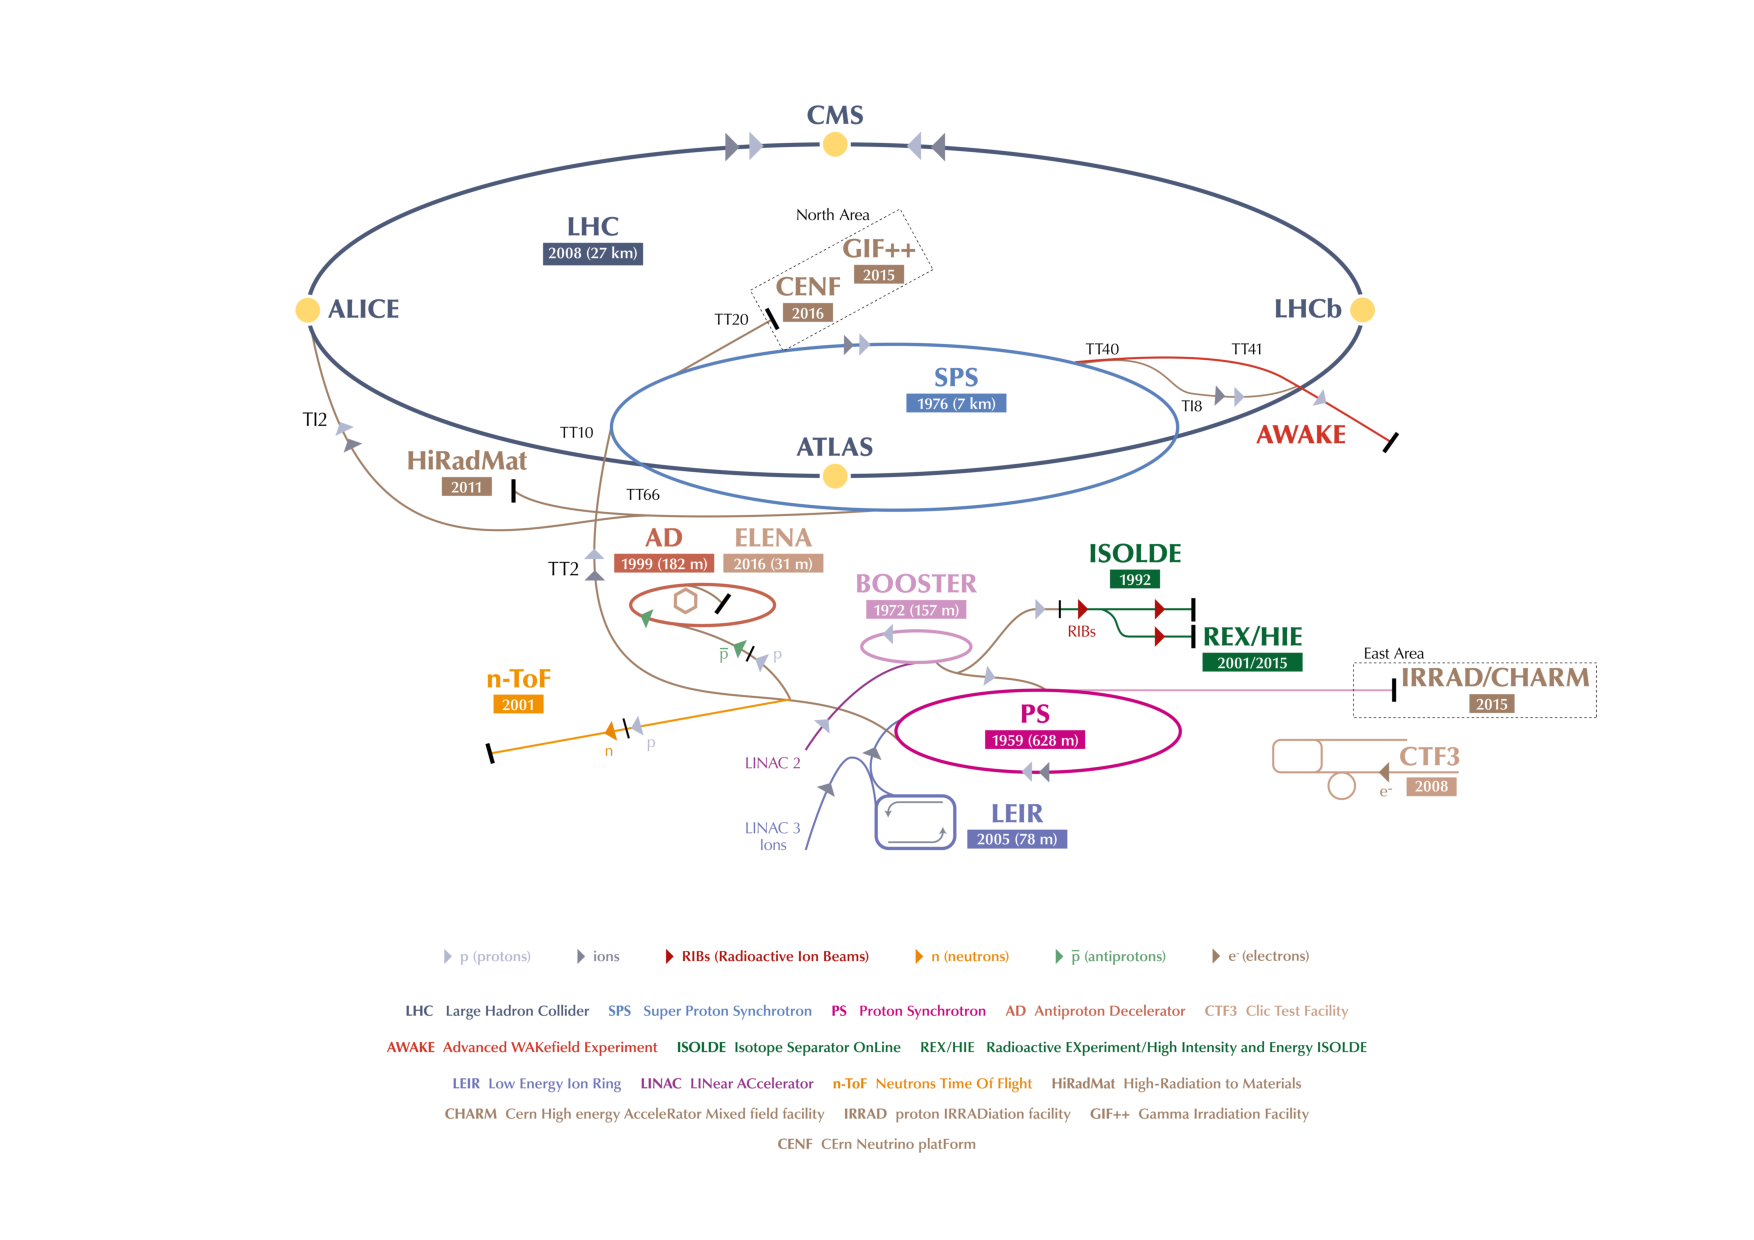
\includegraphics[width=1.15\textwidth,height=19cm]{figures/LHC/CERN_Accelerator_Complex-v2016.jpg}
	\caption{LHC accelerator chain along with all its other experiments which uses proton beam from other parts of accelerator either from PSB, PS or SPS\cite{Fig-CERN-accelerator-complex}}
	\label{fig:CERN-accelerator-complex}
\end{figure}
%%%%%%%%%%%%%%%%%%%%%%%%%%%%%%%%%%%%%%%%%%%%%%%%%%%%%%%%%%%%%%%%%%
%%%%%%%%%%%%%%%%%%%%%%%%%%%%%%%%%%%%%%%%%%%%%%%%%%%%%%%%%%%%%%%%%%
\subsection{Magnet System}
As the LHC is a circular collider; magnet system is one of the core parts and gives particles a circular trajectory in the LHC beam pipes. To be economical LHC has been made in eight arcs and eight straight sections instead of a perfect circle. Apart from bending the beam, it is also necessary to focus the two proton beams this is accomplished using a pair of quadrupole magnets, where the first magnet focus the magnet while other focuses the beam height as shown in Figure~\ref{fig:QuadrupoleMagnet}. A total of 858 quadrupole magnets are installed in LHC to keep the beams focused. Sextuple magnets are also used for proper focusing as every proton in the beam is not exactly with the same energy and on the same path. Several other magnetic multi-poles are used to keep the beam focused  in case the beam suffers from gravitational interactions over protons, electromagnetic interactions among bunches, electron clouds from pipe wall, and so on. Different types of magnets used in LHC are listed here \cite{WebLink:LHC_magnets}. Besides, there are eight sets of ``inner triplets" used at the four interaction points (IPs) to focus the beams during the collisions, to increase the luminosity. The size of bunch goes from 0.2 mm to 17 $\mu m$ at the interaction point of ATLAS or CMS. At the interaction point of ALICE or LHCb it is 71 $\mu m$. Summary of important parameters of LHC is given in Table~\ref{table:LHC-parameters}.
\begin{figure}[!htbp]
	\centering
	\includegraphics[width=0.65\textwidth]{figures/LHC/quadrupole_magnet_pair.png}
	\caption{Pair of quadrupole magnets.}
	\label{fig:QuadrupoleMagnet}
\end{figure}
% \begin{figure}[!htbp]
% 	\centering
% 	\includegraphics[width=0.95\textwidth]{figures/LHC/sextupole-octupole.jpg}
% 	\caption{Sextupole and octupole}
% 	\label{fig:sextupole-octupole}
% \end{figure}



\begin{table}
\vspace{-5.2em}
\centering
\begin{tabular}[!htbp]{l c}
\hline
{\bf Parameters} & {\bf Value} \\
\hline
Circumference of LHC ring   &   26658.883 m \\
\hline
Maximum dipole magnetic field   & 8.33 T \\
Dipole operating temperature    & 1.9 K \\
\hline
Maximum stored energy per beam (nominal) &   362 MJ \\
Maximum stored energy per beam  (2012) &   143 MJ \\
Maximum stored energy per beam  (2016) &   266 MJ \\
\hline
Beam energy at Injection    & 450 GeV \\
Beam energy at collision (nominal) &    7 TeV \\
Beam energy at collision (2012)     &   4 TeV \\
Beam energy at collision (2016)     &   6.5 TeV \\
\hline
Maximum instantaneous luminosity (nominal)  &   $10^{34}$ cm$^-2$ s$^{-1}$ \\
Maximum instantaneous luminosity (2012)     &   $7.7 \times 10^{33}$ cm$^-2$ s$^{-1}$ \\
Maximum instantaneous luminosity (2016)     &   $1.4 \times 10^{34}$ cm$^-2$ s$^{-1}$ \\
\hline
Number of bunches per proton beam (nominal) &   2808 \\
Number of bunches per proton beam (2012)    &   1380 \\
Number of bunches per proton beam (2016)    &   2076 \\
Maximum number of protons per bunch         &   $1.6 \times 10^{11}$ \\
\hline
Protons/bunch (average at start of collision) (nominal)   &   $1.15 \times 10^{11}$ \\
Protons/bunch (average at start of collision) (2012)  &   $1.5 \times 10^{11}$ \\
Protons/bunch (average at start of collision) (2016)  &   $1.1 \times 10^{11}$ \\
\hline
Bunch collision frequency (nominal)         &   40 MHz  \\
Bunch collision frequency (2012)            &   20 MHz  \\
Bunch collision frequency (2016)            &   40 MHz  \\
\hline
Bunch length (at injection)   &   1.7 ns \\
Bunch length (at collision)   &   1.05 ns \\
Energy spread (at injection)   &   1.9$\times 10^{-3}$ \\
Energy spread (at collision)   &   0.45$\times 10^{-3}$  \\
\hline
Half crossing angle  (nominal)   & 143 $\mu rad$ \\
Half crossing angle  (2012)   & 146 $\mu rad$ \\
Half crossing angle  (2016)   & 185 $\mu rad$ \\
\hline
$\beta *$  (nominal) &   0.55 m\\
$\beta *$   (2012)&   0.6 m\\
$\beta *$   (2016)&   0.4 m\\
\hline
RMS beam size at IP1 \& IP5 &   17 $\mu m$ \\
RMS beam size at IP2 \& IP8 &   71 $\mu m$ \\
\hline
$\epsilon_n$(transverse emittance, RMS, normalized) (at injection) &   3.5 $\mu$m\\
$\epsilon_n$(transverse emittance, RMS, normalized) (at collision point) &   3.75 $\mu$m\\
\hline
total longitudinal emittance (at injection) & 1.0 eVs \\
total longitudinal emittance (at collision) & 2.5 eVs \\
\hline
Average mean pile-up (nominal) &   25 \\
Average mean pile-up (2012) &    21 \\
Average mean pile-up (2016) &    27 \\
\hline
Energy loss per turn at 14 TeV              &   7 keV   \\
Energy loss per turn for electrons at 104.6 GeV          &  40,000 keV     \\
% synchtron radiation for electrons: Reference: Particle Physics Experiments at high energy colliders by John Hauptman
\end{tabular}
\caption{LHC technical parameters for proton-proton collisions: nominal, 2012 and 2016 values.\cite{Bruce2016, Schoerner-Sadenius2015, LHC-parameters-2016, LHC-tdr-vol1, cms-lumi-public-results}.}
\label{table:LHC-parameters}
\end{table}

%%%%%%%%%%%%%%%%%%%%%%%%%%%%%%%%%%%%%%%%%%%%%%%%%%%%%%%%%%%%%%%%%%
%%%%%%%%%%%%%%%%%%%%%%%%%%%%%%%%%%%%%%%%%%%%%%%%%%%%%%%%%%%%%%%%%%
\subsection{Key requirements of a particle accelerator} % (fold)
\label{sub:few_key_requirements}

The HEP collider is characterised based on two parameters centre of mass energy and the luminosity. The production rate of heavier particles like Higgs increases with the centre of mass energy. The luminosity is proportional to the number of events per second so it should be maximised. Luminosity is defined as:
\begin{equation}
    L = \frac{k_bN_b^2f_{rev}\gamma}{4 \pi \epsilon_n \beta^*}
\end{equation}
Where,\\
\hspace{2 cm}$k_b$ is the number of bunches per ring,\\
\hspace{2 cm}$N_b$ is the number of protons per bunch,\\
\hspace{2 cm}$f_{rev}$ the revolution frequency,\\
\hspace{2 cm}$\epsilon_n$ is the normalised RMS transverse beam emittance (same in both )\\
\hspace{2 cm}$\beta^*$ is the beta-function at the interaction point\\

Based on the definition of luminosity, we can maximise it by following ways:
\begin{itemize}
    \item By decreasing beam emittance, $\epsilon_n$.
    \item By improving the cryogenic system: As the factor $k_b.N_b$ is limited by thermal energy produced by synchrotron radiation.
    \item By decreasing beam-beam effect~\cite{Herr2014,Papotti2014}. As it scales with $N_b/ \epsilon_n$ which causes the spread in betatron tunes~\cite{Dubouchet2013}.
    \item Also, the space charge~\cite{Oeftiger2016} scales with $N_b/ \epsilon_n$.
\end{itemize}
% subsection few_key_requirements (end)

% section the_large_hadron_collider (end)

%%%%%%%%%%%%%%%%%%%%%%%%%%%%%%%%%%%%%%%%%%%%%%%%%%%%%%%%%%%%%%%%%%
\section{Experiments at the LHC} % (fold)
\label{sec:experiments_at_the_lhc}

At the LHC there are four IPs where the two proton beams are made to collide. At every IP one detector is placed. They are ATLAS, CMS, ALICE, and LHCb as shown in Figure~\ref{fig:LHCgeometry}. Also, there are two more small detectors LHCf and TOTEM installed close to the IP of the two main detectors ATLAS and CMS respectively.
\begin{figure}[!htbp]
	\centering
	\includegraphics[width=0.81\textwidth]{figures/LHC/lhc-schematic.jpg}
	\caption{LHC geometry with arcs and straight sections.}
	\label{fig:LHCgeometry}
\end{figure}
\newline
{\bf ATLAS} (A Toroidal LHC Apparatus) and {\bf CMS} (Compact Muon Solenoid) are the two large general-purpose\footnote{Here, general purpose means this machines will be used for many different kind of physics searches.} detectors having similar design and goal. CMS detector have been described in detail in Section~\ref{sec:cms_experiment}. The main difference in the two is in their magnet systems. This is motivated by the momentum resolution of muons. The momentum resolution for muons, $\Delta p_T/p_T$, is proportional to  $B^{-1}L^{-2}$, where B is magnetic field and L is the lever arm defined as the distance of momentum measurement from the IP of detector. So, to improve the momentum resolution there are two possible choices.

\begin{enumerate}
	\item Increase the magnetic field with compact design, or
	\item Work with low magnetic field with long lever arm
\end{enumerate}

There is also a third possibility to improve the momentum resolution by increasing the leaver arm as well as magnetic field, but it increases the cost of the detector by several factors. So, CMS chooses the first point, i.e., to increase the magnetic field with compact design\footnote{This is why there is word {\bf compact} in the name of CMS.} while ATLAS chooses the design with low magnetic field with long lever arm.

% ATLAS has an eight toroidal magnets combined with a smaller inner solenoid while CMS has a powerful solenoid magnet only.

{\bf ALICE} (A Large Ion Collider Experiment) is a heavy-ion detector. It is specially designed for the study of strongly interacting matter at high densities in quark-gluon plasma phase.

{\bf LHCb} (Large Hadron Collider beauty) is made asymmetrically with respect to the IP of the detector. It is designed specially to investigate the matter-antimatter asymmetry through the study of b-quarks.

{\bf LHCf} (Large Hadron Collider forward) and {\bf TOTEM} (TOTal cross-section, Elastic scattering and diffraction dissociation Measurement at the LHC) are there for the study of forward physics\todo[fancyline]{define forward physics}.
% section experiments_at_the_lhc (end)

% %%%%%%%%%%%%%%%%%%%%%%%%%%%%%%%%%%%%%%%%%%%%%%%%%%%%%%%%%%%%%%%%%%
\section{CMS Detector} % (fold)
\label{sec:cms_experiment}
The design and components of a HEP detector depends upon the physics goals and operation parameters of the particle accelerator. In case of the CMS detector, following challenges are imposed from the LHC:
\begin{itemize}
	\item \textbf{High luminosity:} A high value of  delivered luminosity that implies every-time the two proton bunches cross each other there will be more than one p-p interactions\footnote{More than one p-p interaction in one bunch crossing is known as pile-up. It can be theoretically estimated as the product of inelastic p-p cross-section ($\sigma_{inel}$), instantaneous luminosity ($L$) and the mean time interval between two collision, ($< t >$). \begin{equation}
		mean~pile-up = \sigma_{inel} \times L \times <t>
	\end{equation}}. Given this, there will be more than $\mathcal{O}(1000)$ particles passing through detector during every p-p collision. Thus, the detector should be highly granular which results in increased number of readout channels that should be synchronised with LHC clock.
	\item \textbf{Response time:} At LHC, the two proton beams cross each other every 25 ns. So, the response time of all the sub-detector systems should be less than 25 ns.
	\item \textbf{Radiation hardness:} At every 25 ns the detectors are bombarded with more than 1000 particles so all the sub-detectors should be radiation hard including its electronics, cables, glue, screws, and so on.
\end{itemize}

Restrictions imposed on detector from the physics goals of the LHC:

\begin{itemize}
	\item Good muon identification and momentum resolution ($\approx$ 1\% at 100 GeV).
	\item Efficient triggering and tracking of b-jets and $\tau$'s.
	\item Highly efficient and granular electromagnetic calorimeter to detect and measure energies of electrons and photons.
	\item Good missing transverse energy resolution and di-jet mass resolution requires a ``hermetic'' hadron calorimeter with full geometric coverage and fine lateral segmentation.
\end{itemize}

% When the two beam of proton collides then thousands of particles are produced and out of them only 9 particles are of interest from detector construction point of view. They are photons ($\gamma$), electrons ($e$), muons ($\mu$), pions ($\pi^{\pm}$), kaon ($K^{\pm},~K_L,~K_S$), protons ($p$), and neutrons ($n$). Out of rest there are three neutrinos which interacts only weakly that do not interact in light mass HEP detectors and others are short lived particles. So, 

Based on the above conditions CMS detector is designed in a cylindrical shape having each detector on top of the other with beam pipe at the centre. To have a full geometric coverage, it is designed with a barrel region and two endcap regions. Main part of the CMS detector is its superconducting magnet system, capable of producing a highly uniform magnetic field of 4T to accurately measure the high momentum particles, while the muon detector system are kept outside the magnet but sandwiched in its return yoke. While the tracking system and calorimeters are placed inside the magnet. CMS detector design is shown in Figure~\ref{fig:CMS-detector}.
\begin{figure}[!htbp]
	\centering
	\includegraphics[width=0.95\textwidth]{figures/LHC/cms_120918_03.png}
	\caption{CMS detector drawing}
	\label{fig:CMS-detector}
\end{figure}

\subsection{Coordinate System} % (fold)
\label{sub:coordinate_system}
Right handed coordinate system is used at the CMS detector, having origin at the nominal IP (Figure~\ref{fig:cms-coordinate-system}). Z-axis is considered along the beam direction in such a way so that x-axis will point radially to the centre of LHC ring and y-direction is pointing upwards. The azimuthal angle, $\phi$, is measured in the x-y plane from x-axis and the polar angle, $\theta$, is measured from the z-axis. Instead of describing a particle at some polar angle we prefer to use the variable pseudo-rapidity. It is defined as 
\begin{equation}
	\eta = -ln\bigg[tan\Big(\frac{\theta}{2}\Big)\bigg]
\end{equation}
In the hadron collider use of pseudo-rapidity was motivated from the invariance of its difference, $\Delta \eta$, with respect to the particle boost direction. Also, the particle density remains constant in barrel region of the detector, measured in equal rapidity intervals.

\begin{figure}[htbp]
	\centering
	\includegraphics[width=0.95\textwidth]{figures/LHC/CMS-coordinate-system.png}
	\caption{Right handed coordinate system used by CMS.}
	\label{fig:cms-coordinate-system}
\end{figure}

% subsection coordinate_system (end)
%%%%%%%%%%%%%%%%%%%%%%%%%%%%%%%%%%%%%%%%%%%%%%%%%%%%%%%%%%%%%%%%%%
%%%%%%%%%%%%%%%%%%%%%%%%%%%%%%%%%%%%%%%%%%%%%%%%%%%%%%%%%%%%%%%%%%
\subsection{CMS sub-systems} % (fold)
\label{sub:cms_sub_systems}

%%%%%%%%%%%%%%%%%%%%%%%%%%%%%%%%%%%%%%%%%%%%%%%%%%%%%%%%%%%%%%%%%%
%%%%%%%%%%%%%%%%%%%%%%%%%%%%%%%%%%%%%%%%%%%%%%%%%%%%%%%%%%%%%%%%%%
\subsubsection{Magnet} % (fold)
\label{ssub:magnet}
Magnet system of CMS consists of a superconducting solenoid magnet which is 12.5 m in length and has an inner diameter of 6m. The size of solenoid is large as the tracker, electromagnetic calorimeter and hadron calorimeter are placed inside the solenoid. In barrel region it generates homogeneous magnetic field of 3.8 T. The high magnetic field ensures the appropriate bending power for the highly energetic charged particles to precisely measure their momentum. Outside the solenoid iron yoke is placed for the returning magnetic field. The magnetic field strenght inside the iron yoke is 2 T. Figure~\ref{fig:CMS-magnet} shows the CMS magnet.

\begin{figure}[!htbp]
	\centering
	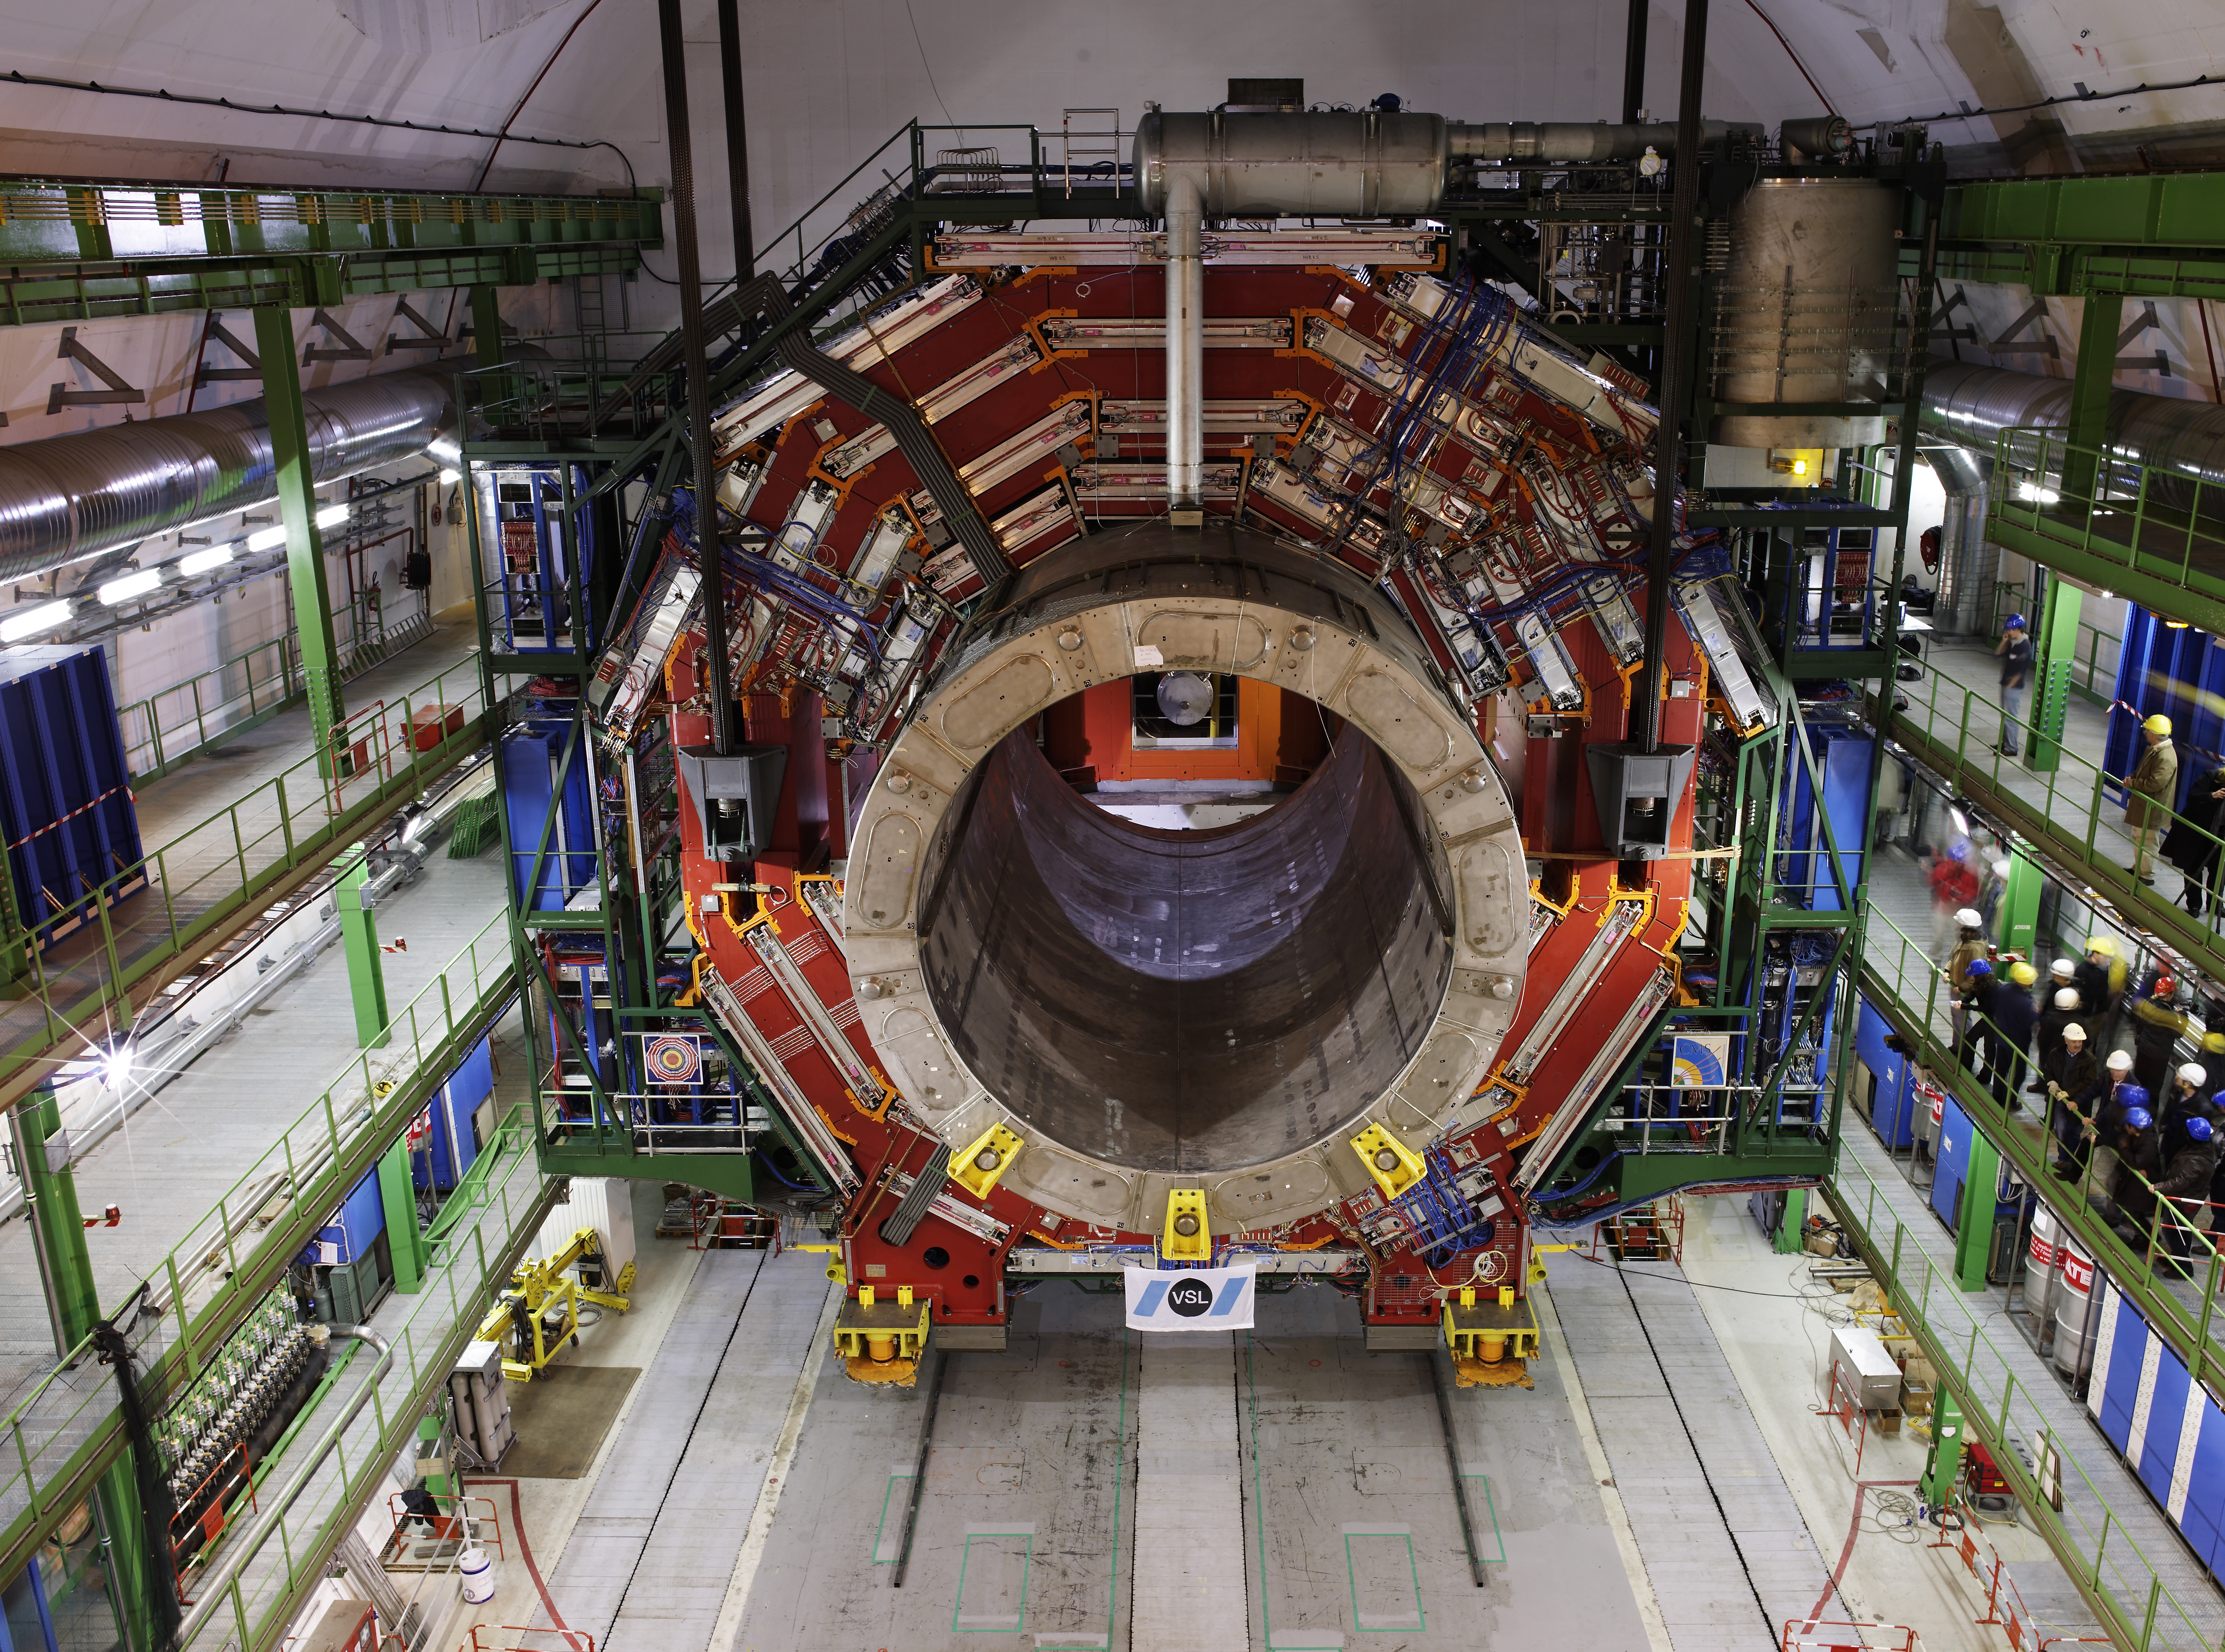
\includegraphics[width=0.95\textwidth]{figures/LHC/CMS_magnet.jpg}
	\caption{CMS Magnet system}
	\label{fig:CMS-magnet}
\end{figure}

% subsubsection magnet (end)
%%%%%%%%%%%%%%%%%%%%%%%%%%%%%%%%%%%%%%%%%%%%%%%%%%%%%%%%%%%%%%%%%%
%%%%%%%%%%%%%%%%%%%%%%%%%%%%%%%%%%%%%%%%%%%%%%%%%%%%%%%%%%%%%%%%%%
\subsubsection{Tracker} % (fold)
\label{ssub:tracker}
Tracker is the first detector that encounters the particles emerging from the p-p collisions. Its purpose is to measure precisely the tracks of all charged particles crossing it. Also, it helps to reconstruct the secondary vertices to tag heavy flavour particles like b-jets or tau leptons. The particle rate is highest in the tracker. So, it should be highly granular and response time should be fast. This condition results in high density of on-detector electronics and this implies a large amount of materials that conflicts with the aim of low material to reduce the multiple scattering, bremsstrahlung, photon conversion and nuclear interactions. Thus, the type, design and number of layers of tracker is the trade-off between the performance, the amount of material, and the cost. Considering these things in mind CMS collaboration decided to have first three layers of silicon pixel detector to precisely measure the primary vertex, secondary vertex and the impact parameter with a total surface area of 1 $m^2$ and 66 million pixels followed by 10 layers of  silicon micro-strip detector covering a total area of 200 $m^2$. Tracker has length of 5.8 m and outer diameter 2.6 m and acceptance is up to $|\eta|<2.5$. Tracker's cross sectional view is shown in Figure~\ref{fig:tracker-cross-section}.

\begin{figure}[!htbp]
	\centering
	\includegraphics[width=0.95\textwidth]{figures/LHC/tracker-cross-section.png}
	\caption{Systematic cross section view of CMS tracker showing silicon pixel and strip detectors. Double line shows back-to-back modules that delivers stereo hits.}
	\label{fig:tracker-cross-section}
\end{figure}
% subsection tracker (end)

%%%%%%%%%%%%%%%%%%%%%%%%%%%%%%%%%%%%%%%%%%%%%%%%%%%%%%%%%%%%%%%%%%
%%%%%%%%%%%%%%%%%%%%%%%%%%%%%%%%%%%%%%%%%%%%%%%%%%%%%%%%%%%%%%%%%%

\subsubsection{Calorimetry} % (fold)
\label{ssub:calorimetry}
In general, the calorimeter is a device that measures the energy of particles by absorbing. The CMS detector uses two different type of calorimeter based on their interaction. They are Electromagnetic CALorimeter (ECAL) and Hadronic CALorimeter (HCAL). ECAL as the name suggest it is designed to measures the particles (electrons and photons) that primly interact via electromagnetic interaction while HCAL is designed to measure particles that interact via strong nuclear interactions.\\\\
ECAL is placed after tracker for the detection of  electrons and photons. It is a homogeneous calorimeter made from lead tungstate ($PbWO_4$) crystals, having a coverage up-to $\eta < 3.0$ including pre-shower system in forward region. The scintillation produced in barrel region is detected by Avalanche photo-diodes and in endcaps it is collected by vacuum photo-triodes. In terms of radiation length\footnote{Radiation length is defined as the mean length travelled by particle to reduce its energy by the factor of 1/e.}, $X_0$, its thickness is 25$X_0$ which guarantees almost full shower containment.\\\\
In between ECAL and magnet system, brass/scintillator sampling HCAL with coverage up to $\eta < 3.0$ is placed. To have a full geometric coverage HCAL is extended up to $\eta < 5.0$ using forward sampling iron/quartz-fibre calorimeter. This is crucial to measure the (missing) transverse energy of the event.

% The energy resolution of the ECAL can be parameterized  
% subsubsection calorimetry (end)


%%%%%%%%%%%%%%%%%%%%%%%%%%%%%%%%%%%%%%%%%%%%%%%%%%%%%%%%%%%%%%%%%%
%%%%%%%%%%%%%%%%%%%%%%%%%%%%%%%%%%%%%%%%%%%%%%%%%%%%%%%%%%%%%%%%%%
\subsubsection{The Muon System} % (fold)
\label{sub:the_muon_system}
From the name of CMS detector it is evident that the precise detection of muons is one of its main target. It is motivated by the presence of muons in the final state of many interesting physics processes, such as, the decay of Higgs boson into ZZ which subsequently decay in four leptons and especially, the case where all 4 leptons are muons is refereed to as the ``gold plated'' channel as we can detect muons efficiently over higher background contributions at LHC. At CMS, muon system serves three different functions viz. identification, momentum measurement and triggering of muons. The strong superconducting magnet system with its return yoke of CMS, helps to acquire good momentum measurement and triggering capabilities. The return yoke of magnet system also serves as the hadron absorber. Only muons leave their tracks in the muon detector system, as all other particles are already absorbed by the calorimeters. Thus, the appearance of charged particle in the muon system signifies that it can only be muons. The track left by muon in the CMS detector is illustrated in Figure~\ref{fig:muon-system-cross}. 
\begin{figure}[!htbp]
	\centering
	\includegraphics[width=0.55\textwidth]{figures/LHC/MuStations.png}
	\caption{A muon leaves curved trajectory in LHC and the bending changes as the magnetic field direction of solenoid inside and outside are opposite.}
	\label{fig:muon-system-cross}
\end{figure}
The layout of the CMS muon detector system is shown in Figure~\ref{fig:muon-system-layout}. Three different types of gaseous detectors used for the muon system which were chosen based on the background level, muon rate, uniformity and magnitude of magnetic field. Drift tubes are used as tracking detector in the barrel region with relatively lower magnetic field intensity and which have lower background rates as compared to the endcaps. 
For the endcap regions Cathode Strip Chamber (CSC) are employed as they are provide precise information about muons momentum and time information even in high radiation environment. The pseudo-rapidity coverage of DTs is $|\eta|<1.2$ and for CSCs is $0.9<|\eta|<2.4$. Along with DTs and CSCs, Resistive Plate Chamber (RPC) detectors are also installed to have a fast dedicated  muon triggering system in both barrel and endcap region up to $|\eta|<1.6$~\cite{muon-tdr}. The CMS muon detector system covers the geometric region up-to $|\eta|<2.4$ but RPCs are deployed up-to $|\eta|<1.6$ as RPCs cannot withstand the radiation level after pseudo-rapidity region of 1.6. Thus to reconstruct muons in pseudo-rapidity region higher than 1.6, CMS collaboration decided to employ Gas Electron Multiplier (GEM) detectors in region  $1.6<|\eta|<2.2$, which is able to provide good space resolution and time resolution even in high environment radiation during Long Shutdown-2 (LS2, 2019-2020). The pseudo-rapidity range is limited to $|\eta|<2.2$ because of space constrains. GEM  detectors are described in details in Chapter~\ref{ch:gem}.
\begin{figure}[!htbp]
	\vspace{-3.2em}
	\centering
	\includegraphics[width=0.85\textwidth]{figures/LHC/pictures_MuonSys-mod3.png}
	\caption{Longitudinal layout of one quadrant of the CMS detector. There are four DT stations named MB1-MB4 marked with green colour. Four CMS system in high pseudo-rapidity region named ME1-ME4 in blue colour. Also, there are several RPC stations in barrel region and part of endcap region marked with red colour.}
	\label{fig:muon-system-layout}
\end{figure}
Summary of CMS detector sub-system including its main characteristics and composition is given in Table~\ref{table:CMSMainChar}.
% subsection the_muon_system (end)
% subsection cms_sub_systems (end)
% % section cms_experiment (end)

\begin{table}
% \vspace{-5.2em}
\centering
\begin{tabular}[!htbp]{l l l}
\hline
{\bf Sub-system} & {\bf Composition} & {\bf Charateristics} \\
\hline
Tracker  & silicon strip and  & isolated track effiency $\epsilon > 95\%$ \\
	& pixel detector	& within jets $\epsilon \sim 90\%$ \\
	& 	& primary vertex resolution: 10-20 $\mu m$ \\
	& 	& $p_T$ resolution: $\Delta p_T/p_T = 1\%$ (0.1 TeV), 10\% (TeV)\\
	& 	& coverage $\eta<2.5$ \\
\hline
ECAL 	& 	$PbWO_4$ crystals 	& energy resolution:\\
		& 	& $\big(\frac{\sigma}{E}\big)^2 = \big(\frac{2.7\%}{\sqrt{E}}\big)^2 + \big(\frac{210}{E}\big)^2 + 0.55\% $  (barrel)\\
		& 	& $\big(\frac{\sigma}{E}\big)^2 = \big(\frac{5.7\%}{\sqrt{E}}\big)^2 + \big(\frac{245}{E}\big)^2 + 0.55\% $  (end-caps)\\
		& 	& coverage $\eta < 3$ \\
\hline
HCAL 	& 	Cu-Zn 	& energy resolution:\\
		& 	scintillators & $\big(\frac{\sigma}{E}\big)^2 = \big(\frac{68\%}{\sqrt{E}}\big)^2 + 4.5\%$ \\
		& 	& coverage $\eta < 3$ \\
\hline
Muon system & gaseous & efficiency $\epsilon \sim 98\%$ \\
			& detectors & $\Delta p_T/p_T =$8-15 \% (0.01 TeV)/20-40\% (TeV)\\
		& 	& coverage $\eta < 2.4$ \\
\hline
\end{tabular}
\caption{Main characteristics of the CMS sub-system~\cite{JeremieThesis}}
\label{table:CMSMainChar}
\end{table}


% %%%%%%%%%%%%%%%%%%%%%%%%%%%%%%%%%%%%%%%%%%%%%%%%%%%%%%%%%%%%%%%%%%
\subsection{CMS Trigger and Data Acquisition system} % (fold)
\label{sub:cms_trigger_and_data_acquisition_system}
The LHC produces 1 billion p-p collisions every second and thousands of particles produced during these collisions cross the CMS detector and reconstruction of these events generates several Terabytes of data. However, till now we neither have a switch with the required bandwidth that can transfer enormous data for further processing nor the disk space to store all of them. Even if we have one, then there are only a few fractions of data that are interesting for new physics or help to understand the existing one as most of the collisions is the low-energy glancing collision instead of head-on interaction. The maximum amount of data that can be stored every day is of the order of few Terabytes that decides the rate at which we can accept the events ($\sim$ 100 Hz).The concept of the trigger, method to select events of interest, was first introduced by ZEUS experiment~\cite{ZEUSCollaboration1993}, that handles data in real time, coupled with complex data acquisition system. While designing the trigger one has to keep in mind that trigger should efficiently accept the interesting physics while rejecting the non-interesting ones as whatever information lost at this level can not be recovered.

The CMS trigger system is divided into two steps, level 1 (L1) trigger which is a custom hardware process running synchronously with the LHC bunch crossing frequency of 40 MHz and the High-Level Trigger (HLT)~\cite{paper:JINST:CMSCollaboration}. The L1 trigger system analyses the events based on the information of calorimeter and muon system and  then selects the interesting events. However, this decision cannot take place within 25 ns, so a latency of 3.2 $\mu s$ was added. The maximum allowed frequency at the L1 stage is 100 kHz. Then the complete information is sent to HLT processing farm to reduced the event rate to $\sim$100 Hz. The remaining information is sent to Tier-0 centres to store and use it for offline analysis.



% section cms_trigger_and_data_acquisition_system (end)

% %%%%%%%%%%%%%%%%%%%%%%%%%%%%%%%%%%%%%%%%%%%%%%%%%%%%%%%%%%%%%%%%%%
\subsection{CMS Offline Computing} % (fold)
\label{sub:cms_offline_computing}
Once the data are selected by the trigger system, they are ready to be analysed offline. Before that, the raw data need to be processed, i.e., to convert data into understandable physics objects like electrons, muons, photons, jets, and so on. This step is known as object reconstruction which is the most CPU intensive task in the data processing chain of CMS. In this step one needs to reconstruct the primary vertices, charged particle tracks, identify electrons, photons, muons, reconstruct jets, apply b-tagging algorithm to reconstruct b-jets, run detector specific filtering and so on.
To perform all these steps CMS developed its software which is known as CMSSW. This software is based on Event Data Model (EDM) centred around the concept of the event. Here, an event is a C++ object container for all raw and reconstructed data related to a particular collision. Finally, these events are stored in ROOT files~\cite{Root1996}. The CMSSW event processing model consists of one executable called cmsRun, and many plug-in modules. These modules contain all the necessary codes for the event processing such as calibration and reconstruction algorithms~\cite{Bayatyan2005}.
To analyse data, we also need MC simulations which are carried out based on the predictions of SM and various new physics models. MC events are generated at parton level. Then showering and hadronization is applied, and finally, these events are put through the GEANT4~\cite{Agostinelli2003} based CMS detector simulation. The result is data similar to what one obtains from the actual detector. This MC data can then also be reconstructed as if it were  detector data.


% section cms_offline_computing (end)




% \begin{figure}[!htbp]
% 	\centering
% 	\includegraphics[width=0.95\textwidth]{figures/lumi-proj-2016-final-v2}
% 	\caption{The integrated luminosity of the LHC with proton-proton collisions in 2016 compared to previous years. Luminosity is a measure of a collider’s efficiency and is proportional to the number of collisions. The integrated luminosity achieved by the LHC in 2016 far surpassed expectations and is double that achieved at a lower energy in 2012. (Image : CERN)\todo[inline]{Update the caption.}}
% 	\label{fig:lumi-proj-2016-final-v2}
% \end{figure}





% Because of limited geometrical space in LHC ring the beam pipe was designed as a ``twin-aperture" magnets, where superconducing ring is housed in a common return yoke and cryostat.

% chapter the_lhc_and_cms_machine (end)


% \begin{figure}[!htbp]
% 	\centering
% 	\includegraphics[width=0.95\textwidth]{figures/LHC/cms_complete_labelled.png}
% 	\caption{CMS detector drawing}
% 	\label{fig:CMS-detector-2}
% \end{figure}

  \chapter{Gas Electron Multiplier} % (fold)
\label{cha:gas_electron_multiplier}

\section{Introduction} % (fold)
\label{sec:introduction}

% section introduction (end)
The invention of Multi-Wire Proportional Chamber (MWPC) in 1968 by Georges Charpak was one of breakthrough in gaseous detectors, since it had better rate capability vis-a-vis its predecessors~\cite{Charpak1968}. 
This invention was also led to Nobel prize to George Charpak in 1992. With time the design and performance of MWPC have been improved. But because of our increasing demands with the acquired knowledge its limitation reached in terms of the maximum rate capability and granularity. In 1988 Anton Oed invented the Micro-Strip Gas Counter (MSGC). 
This detector had overcome the rate limitation due to positive-ion accumulation in the gas volume and able to reach up to few tens of micron in position resolution. 
Also, it can sustain the particle flux exceeding the $MHz/mm^2$ range. Its performance was very impressive but long-term study revealed its two weakness. They are:
\begin{enumerate}
	\item Formation of deposits on the electrodes, which affects the gain and age of the detector.
	\item In presence of highly ionizing particles sometimes a destructive discharge happens.
\end{enumerate}
The invention of Micro-Pattern Gaseous Detector (MPGD) focuses these issues. 
It has unprecedented spatial resolution, large sensitive area, high rate capability, operational stability along with long life-time in particular the Gas Electron Multiplier (GEM)~\cite{Sauli1997,Sauli1999} detectors. 
Several new study also shown that if a reasonable precaution are taken on the component quality it might be less vulnerable to the radiation induced ageing than the standard silicon micro-strip detectors~\cite{TITOV2004,Titov2002}.

% \section{GEM Introduction \& Operational Principle} % (fold)
% \label{sec:gem_introduction_&_operational_principle}
GEM is a new concept from Fabio Sauli at CERN \cite{Sauli1997}. It was introduced to improve the performance of microstrip gas chamber and to match the harsh running conditions of experiments at CERN's LHC collider, where detectors will have to cope with high data rates and will be exposed to intense bombardment by high-energy particles \cite{detector:1732870}.

It is a thin plastic sheet coated with metal on both sides and chemically pierced by a regular array of holes a fraction of a millimetre across and apart. 
Applying a voltage (about 500V on 50$\mu$) across the GEM conducting layers, the resulting high electric field in the holes makes an avalanche of ions and electrons pour through each. 
The GEM foil is shown in Figure \ref{fig:gem}.
\begin{figure}[!htbp]
	\centering
	\includegraphics[width=0.95\textwidth]{figures/GEM/KEKDTP3.jpg}
	\caption{(Left) The gas electron multiplier (GEM) foil can image two-dimensional position of particles passing through a gaseous chamber. (Right) The cross sectional view of the GEM shows strong electric fields in the vicinity of holes where electron signals are amplified.}
	\label{fig:gem}
\end{figure}
The region inside GEM detector have three different regions: drift electrode, a conversion and drift region.
%, a GEM mesh collecting and multiplying the charge in a gas avalanche, and induction gap in which a high electric field is used to extract and drift the electrons towards the collecting electrodes. This is shown in Figure \ref{fig:gemgaps}. 
The large effective gains (up to $10^4$), full efficiency of detection and very good localization accuracies for minimum ionizing particles is promising to us. 
In the thin gap of GEM few tens of primary ion pairs creates; cascading to two GEM meshes so it can provide large gains and better performances with very less probability of discharge~\cite{Bressan1999}.
\begin{figure}[!htbp]
	\begin{center}
		\includegraphics[width=0.95\textwidth]{figures/GEM/triple_gem.png}
		\caption{Illustration of GEM working}
		\label{fig:gemgaps}
	\end{center}
\end{figure} 
% section gem_introduction_&_operational_principle (end)
\section{Fabrication \& Characterization} % (fold)
\label{sec:fabrication_&_characterization}
\subsection{Foil Production}
Through Transfer of Technology (TOT) Micropack signed an agreement for the development of GEM foils in India in collaboration with Indian Institutions. 
After continuous efforts, refining of processes and repeated trials, Micropack has been successful in realizing $10~cm~\times~10~cm$ and $30~cm~\times~30~cm$ GEM foils, meeting the standard dimensional requirements.
Micropack started the production with single mask process as this configuration is the one we are going to use in CMS detector.
But, after several attempts they realized that this is quite challenging so they switched to double mask process. They quickly succeeded in production of the double-mask GEMs.
It is produced in a similar fashion as at CERN PCB workshop~\cite{DEOLIVEIRA2009}.
The foil used by Micropack was 50 $\mu m$ PI (Apical Type NP) film with 5 $\mu m$ copper coating on both side. Figure~\ref{fig:Foil_and_Cone}(a) shows the $10~cm~\times~10~cm$ GEM foil produced by Micropack and the Fig.~\ref{fig:Foil_and_Cone}(b) shows the cross-sectional view of the foil showing the double conical structure.
To qualify these GEM foils as commercially and scientifically reliable, a number of quality control test have to be performed. 
The two main quality control tests are optical test and electrical test. The optical test gives us information about the quality of produced foil like the hole geometry, pitch information and about the defects, if any. 
While the electrical test gives us information about the leakage current, discharge effects, etc.
\begin{figure}[!htbp]
    \centering
    \begin{subfigure}[b]{0.46\textwidth}
        \includegraphics[width=6cm, height=4cm]{figures/GEM/figures/Foil_01.png}\qquad
        \caption{ }
    \end{subfigure}
    \begin{subfigure}[b]{0.46\textwidth}
        \includegraphics[width=6cm, height=4cm]{figures/GEM/figures/double_cone.png}
        \caption{ }
    \end{subfigure}
   \caption{(a) 10 cm $\times$ 10 cm GEM foil encapsulated in a frame and (b) Cross-sectional view of the foil showing the double cone structure of the engraved holes. } \label{fig:Foil_and_Cone}
\end{figure}

\subsection{Optical Assessment}
GEM performance depends heavily on the quality and parameters of GEM foil like thickness of foil, hole diameter, pitch, and defects like missing holes, un-etched areas, excess-etching, burnt areas, etc. 
To check these defects and to measure the hole-size and pitch several method was developed using an automated 2D-CCD scanner~\cite{Posik2015, Becker2006}. 
However we used a different technique. We divided the GEM foil into several sectors and captured a high resolution picture using the AF-S Micro Nikon 40 mm 1:2.8G lens. We used a soft box ($1~m~\times~1~m$) light source for uniform illuminating the GEM foil.
A sketch of the set-up is shown in Fig.~\ref{fig:Optical_Sketch}.
\begin{figure}[!htbp]
    \centering
    %\begin{subfigure}[b]{0.7\textwidth}
        %\includegraphics[width=12cm, height=8cm]{figures/GEM/figures/NIMA_paper_Images001.jpeg}
        \includegraphics[width=12cm, height=8cm]{figures/GEM/figures/2.jpeg}
        %\includegraphics[width=9cm, height=8cm]{figures/GEM/figures/Optical_Sketch.png}
    %    \caption{ }
    %\end{subfigure}
   \caption{Sketch of the set-up used for the optical measurements.}   \label{fig:Optical_Sketch}
\end{figure}
Fig~\ref{fig:Optical_01} shows the found defects in the considered GEM foil. Also, the measured number of defects are shown in Fig.~\ref{fig:Optical_04}.
\begin{figure}[!htbp]
    \centering
    \begin{subfigure}[b]{0.29\textwidth}
        \includegraphics[width=4cm, height=3cm]{figures/GEM/figures/3a.jpg}
        \caption{ }
        \label{fig:O_4a}
    \end{subfigure}
    \begin{subfigure}[b]{0.29\textwidth}
        \includegraphics[width=4cm, height=3cm]{figures/GEM/figures/3b.jpg}
        \caption{ }
        \label{fig:O_4b}
    \end{subfigure}
    \centering
    \begin{subfigure}[b]{0.29\textwidth}
        \includegraphics[width=4cm, height=3cm]{figures/GEM/figures/3c.jpg}
        \caption{ }
        \label{fig:O_4c}
    \end{subfigure}
    \centering
    \begin{subfigure}[b]{0.29\textwidth}
        \includegraphics[width=4cm, height=3cm]{figures/GEM/figures/3d.jpg}
        \caption{ }
        \label{fig:O_5a}
    \end{subfigure}
    \centering
    \begin{subfigure}[b]{0.29\textwidth}
        \includegraphics[width=4cm, height=3cm]{figures/GEM/figures/3e.jpg}
        \caption{ }
        \label{fig:O_5b}
    \end{subfigure}
    \centering
    \begin{subfigure}[b]{0.29\textwidth}
        \includegraphics[width=4cm, height=3cm]{figures/GEM/figures/3f.jpg}
        \caption{ }
        \label{fig:O_5c}
    \end{subfigure}
   \caption{Observed imperfections in the foils: (a) Un-etched area, (b) under-size hole, (c) over-size hole (d) missing hole, (e) excess etching and (f) burnt area.} \label{fig:Optical_01}
\end{figure}

% as shown in the Figures \ref{fig:Optical_02} (a) and \ref{fig:Optical_02} (b), respectively. 
% \begin{figure}[!htbp]
%     \centering
%     \begin{subfigure}[b]{0.44\textwidth}
%         \includegraphics[width=5cm, height=4cm]{figures/GEM/figures/O_1b}
%         \caption{ }
%         \label{fig:O_1a}
%     \end{subfigure}
%     \begin{subfigure}[b]{0.44\textwidth}
%         \includegraphics[width=5cm, height=4cm]{figures/GEM/figures/O_1a}
%         \caption{ }
%         \label{fig:O_1b}
%     \end{subfigure}
%    \caption{(a) Outer holes when front light is ON and (b) Inner holes when back light is ON.} \label{fig:Optical_02}
% \end{figure}
%=====================================================================	
%=====================================================================

\begin{figure}[!htbp]
    \centering
    \begin{subfigure}[b]{0.49\textwidth}
        \includegraphics[width=7.6cm, height=5.5cm]{figures/GEM/figures/Apical_Defects.pdf}\qquad
        \caption{ }
        \label{fig:O_9a}
    \end{subfigure}
    \begin{subfigure}[b]{0.49\textwidth}
        \includegraphics[width=7.6cm, height=5.5cm]{figures/GEM/figures/CopperDefects.pdf}
        \caption{ }
        \label{fig:O_9b}
    \end{subfigure}
   \caption{Number of defects seen in (a) Insulator (Apical Type NP) and (b) Copper, for one of the 10 cm $\times$ 10 cm foil.} \label{fig:Optical_04}
\end{figure}

%=====================================================================

\subsection{Electrical Assessment}
The production quality of GEM foils can be quantified through optical and electrical tests. The optical test gives the information regarding the hole geometry and pitch related information whereas electrical test provides the parameters about the efficacy of the foils and hence is important in determining the quality of GEM foils. 
Electrical properties of the GEM foils were discerned by measuring its leakage current extended over a period of time after proper cleaning using adhesive roller.\tabularnewline
We divide electrical tests mainly in two types, quality control short or fast (QC fast) and quality control long (QC long) as per the CERN standards of quality control classification~\cite{Abbaneo2015}, which requires these two tests to be done in order to qualify these foils. 
The difference between QC fast and QC long lies in applying voltage for shorter or longer periods of time respectively, and monitoring the current. 
The other difference being that the QC fast gives the preliminary idea of leakage current or electrical connectivity of the foil but for more detailed study, QC long provides the behaviour of the foil at high voltages in terms of information regarding the actual leakage current and the number of discharges, if any, for the reasonably longer duration of time. 
Here, both the tests have been performed; the electrical connectivity of the foils by QC fast method has been done with insulation tester MIT Megger 420 \cite{twelve}. Using this test, we established that the foils have good electrical connectivity.
\begin{figure}[!htbp]
    \centering
    %\begin{subfigure}[b]{0.7\textwidth}
        \includegraphics[width=12cm,height=8cm]{figures/GEM/figures/10.jpeg}
        %\includegraphics[width=12.0cm, height=9.0cm]{figures/GEM/figures/Electrical_Sketch.png}
    %    \caption{ }
        %\label{fig:Setup}
    %\end{subfigure}
   \caption{Sketch of the set-up used for the measurement of leakage current.} \label{fig:Cleaning_Measurement}
\end{figure}
%=====================================================================
\begin{figure}[!htbp]
    \centering
    \begin{subfigure}[b]{0.5\textwidth}
        %\includegraphics[width=7.5cm, height=5.5cm]{Indian_foils_H20.pdf}
        \includegraphics[width=7.5cm, height=5.5cm]{figures/GEM/figures/Fig_11(a).pdf}
        \caption{ }
        \label{fig:Indian_foils_H20}
    \end{subfigure}
    \begin{subfigure}[b]{0.46\textwidth}
        %\includegraphics[width=7.5cm, height=5.5cm]{CERN_foils.pdf} 
        \includegraphics[width=7.5cm, height=5.5cm]{figures/GEM/figures/Fig_11(b).pdf} 
        \caption{ }
        \label{fig:CERN_foils}
    \end{subfigure}
   \caption{Leakage Current of (a) Micropack Foils and (b) CERN Foils, at an average temperature of T=27$^{\circ}$C and relative humidity equal to 20\%.} \label{fig:L_01}
\end{figure}
%=====================================================================
%\begin{figure}[!htbp]
%    \centering
%    \begin{subfigure}[b]{0.75\textwidth}
%        \includegraphics[width=10cm, height=7cm]{Combined_foils_H20.pdf}
%        %\caption{ }
%        %\label{fig:Combined_foils_H20}
%    \end{subfigure}
%   \caption{Comparison of Leakage Currents between Micropack and CERN foils taken at different voltages.} \label{fig:Combined_foils_H20}
%\end{figure}
%=====================================================================

For the better precision in the current measurement, Keithley Electrometer 6517B \cite{thirteen} has been used. 
The measurement set-up consists of a bare GEM foil connected to Keithley 6517B pico-ammeter interfaced with a computer via a GPIB interface and the LabView program was used to record the measurements as shown in the Figure \ref{fig:Cleaning_Measurement}. The current measurement range was set from 0 to 200 nA, with an accuracy of $\pm$0.2 $\%$.
The leakage current thus measured as a function of applied voltage is shown in Figure \ref{fig:L_01} (a) for the Micropack foils.
For comparison, the same measurement were also done for foils procured from CERN and the results are shown in the Figure \ref{fig:L_01} (b).  
%Figure \ref{fig:Combined_foils_H20} shows the comparison of leakage current between Micropack and CERN foils as a function of applied voltage. 
The Micropack and the CERN foils were found to show similar results under similar ambient conditions.
However, as the humidity escalates, the leakage current in CERN foils increases more rapidly compared to the Micropack foils.
The maximum current of 12 nA and 25 nA at an applied voltage of 550V, corresponding to the humidity of 40\% has been observed in Micropack and CERN foils respectively. Figure \ref{fig:LvH} shows the leakage current for various applied voltages under different ambient conditions.
From the Figure \ref{fig:LvH}, it can be fairly concluded that humidity does have drastic effects on the leakage current measurement.
Therefore, the current was also measured in nitrogen environment. Since, Nitrogen is the contamination free standard medium as it is relatively inert and neither reacts with stored materials nor carries moisture.
By slowly percolating nitrogen gas into the test enclosure, which in our case was a Plexiglass enclosure in which nitrogen gas was continuously flowing, moisture-laden air was purged out and the current was measured. All the foils showed a current less than 1 nA.
\begin{figure}[!htbp]
	\centering
	\includegraphics[width=0.45\textwidth]{figures/GEM/megger.png}
	\caption{caption}
	\label{fig:label}
\end{figure}
All the measurements were carried out in the clean room of class 100 installed with a KANOMAX dust particle counter Model 3887 \cite{fourteen} which monitors the particle count. Humidity was controlled by dehumidifier installed in the clean room.
The QC long test of the GEM foils were performed by placing foils in a Plexiglass enclosure. After flowing nitrogen continuously for more than two hours, the leakage current was measured in each foil at different voltages in steps of 50V starting from 450V and going up until 600V for time intervals nearly equal to 700s.
At 600V, at most two discharges were seen during the time period of around 700s. The corresponding results are shown in Figure \ref{fig:QC_Long_01}. Similar results were obtained for both other foils as shown in Figure \ref{fig:QC_Long_02}.

% section fabrication_&_characterization (end)

\section{GEM for CMS}
The CMS experiment was designed to have a highly redundant muon system using three detector technologies: DT, CSC and RPC. The endcap regions rely on CSC and RPC for $|\eta|<1.6$. For higher $\eta~ (|\eta|>1.6)$ regions, the system has limited redundancy and only CSC are installed. In the future running of LHC at full luminosity, the particle rate in the forward region is expected to reach several tens of kHz/$cm^2$ and the integrated charge will reach several $C/cm^2$, which make the use of the originally planned RPC technology questionable. To overcome these limitations, the CMS GEM collaboration proposed the GEM as a potential candidate to upgrade the high-$\eta$ region of the forward muon system \cite{Colaleo:2021453}. 
%The CMS muon system was designed as a highly hermetic and redundant muon system, composed of three detection technologies. Precision measurements are provided by \gls{dt} in the barrel, covering acceptances up to $|\eta|<1.2$, and \gls{csc} in the endcaps covering $1.0 < |\eta|<2.4$. \gls{rpc} ensures adequate redundancy and triggering up to $\eta | > 1.6$ where the background particle rates are highest and the bending in the magnetic field is smallest.

The chosen technology are GEM, where amplification occurs in the narrow wholes of a thin kapton foil. Three subsequent stages/foils allow for a reasonable amplification at every stage/foil while providing a high total amplification. Two of such triple-GEM chambers are combined to a so called super chamber.

The proposed upgrade targets the following improvements:
	\begin{itemize}
		\item Re-establish the redundancy in the difficult region beyond $\eta = 1.6 $
		\item Improve tracking performance in the high rate environment
		\item The combined operation of CSC and GEM detectors allows a measurement of the bending angle at trigger level, thus strongly reducing the rate of mis-measured muons driving the triggers rate.
	\end{itemize}

\subsection{GE11 Details}
The aim of the CMS GEM Collaboration is the development and the installation of triple-GEM detectors in the forward region of the CMS muon end-caps during the LS2 upgrade foreseen in 2018. The project is named GE1/1, where ``G'' stands for GEM, ``E'' stands for for End-cap, the first ``1'' corresponds to the first muon station and the second ``1'' the first ring of the station. 144 large trapezoidal chambers will be organized by pair to form super-chambers that will cover the full $\phi$ coordinate and the pseudo-rapidity region 1.6$ < \eta < $2.2.
The detectors will be inserted in front of the ME1/1 station in the slots originally foreseen for RPC detectors as described in Fig.~\ref{fig:GE11pos}. 
\begin{figure}[!htbp]
	\centering
	\includegraphics[width=0.95\textwidth]{figures/GEM/cms_upg_o_g_b_ni_ge1_r_140227.pdf}
	\caption{Cross-sectional view of CMS quadrant showing the location of GEM detectors in red.}
	\label{fig:GE11pos}
\end{figure}
The goal is to complement the CSC system to ensure the good reconstruction and selection efficiency after the high-luminosity upgrade of the LHC, while keeping the L1 trigger to an acceptable rate. 
It is trapezoidal in shape with active area of $990\times (220-445)mm^2$. This size is imposed by the geometry of the vacant high-$\eta$ area in CMS muon endcap. GE1/1 chamber hosts a Triple-GEM detector with a $3/1/2/1~mm$ (drift/transfer 1/transfer 2/induction) electrode gap configuration, as shown in Fig. \ref{GEM:cascade}. The GEM foil ($50\mu m$ thick kapton foil with $5\mu m$ copper on both sides) consists of a thin kapton foil, metal-clad on both side, with a high density of chemically pierced holes. By applying suitable potential difference between two sides, this mesh can act as an amplifier for electrons released by ionization of the gas. The detector readout board is divided into eight $\eta$-partitions with 384 strips each oriented radially along the long side of the detector with a pitch varying from $0.6mm$ (short side) to $1.2mm$ (long side). Each partition is subdivided along the $\phi$-coordinate into three readout sectors with 128 strips or channels each. During test beam we scanned three different sectors of GE1/1, i.e. $(i\eta,i\phi)~=~\{(1,2),(5,2),(8,2)\}$. In Fig. \ref{GE11} red and yellow color shows which sector of GE1/1's are exposed to the beam. Red sectors are taken with gas $Ar/CO_2/CF_4~(45/15/40) $ while yellow sector is taken with gas $Ar/CO_2~(70/30)$.

\begin{figure}[!htbp]
\centering
\includegraphics[width=2.0in]{figures/GEM/GEMCascade.png}
\caption{Generic triple-GEM chamber, showing drift, transfer, and signal induction gap regions within the detector.}
\label{GEM:cascade}
\end{figure}

%\begin{figure}[!htbp]
%\centering
%\includegraphics[width=1.0in]{figures/GEM/GE11.png}
%\caption{Different $(i\eta,i\phi)$ sectors of full size GE1/1 detector prototype.}
%\label{GE11}
%\end{figure}

\begin{figure}[!htbp]
\centering
\includegraphics[width=1.0in]{figures/GEM/GE11.png}
\caption{Different $(i\eta,i\phi)$ sectors of full size GE1/1 detector prototype.}
\label{GE11}
\end{figure}


\subsection{Detector Design Description For Test Beam Analysis}
The full design of the GEM chamber is shown in Figure \ref{fig:ge11}.
\begin{figure}[!htbp]
	\begin{center}
		\includegraphics[width=0.95\textwidth]{figures/GEM/ge11cad.png}
		\caption{Layer by layer view of GEM detector}
		\label{fig:ge11}
	\end{center}
\end{figure} 
The trapezoidal chambers are sectored in $\eta$ partitions to cover $10^0$ each in the azimuthal sector and provide radial readout strip with the strip pointing to the LHC beam pipe (Figure \ref{fig:gemTrapezoidal}). In this design, the strip pitch varies from 0.6 mm (lower side) to 1.2 mm (upper side) with 8-$\eta$ sectors. To improve tracking capabilities, two GEM chambers will be mounted face-to-face to form a double layer called ``Super-Chamber". Thus each Super-Chamber will provide two impact points for each muon track. The gas gap configuration is: 3 mm (drift), 1 mm (transfer1), 2 mm(transfer2), and 1 mm (induction) as shown in Figure \ref{fig:tripple-gem}, which proved to be optimal for timing purposes. The gas mixture is $Ar/CO_2/CF_4~45/15/40$.
\begin{figure}[!htbp]
	\begin{center}
		\includegraphics[width=0.55\textwidth]{figures/GEM/gemTrapezoidal.png}
		\caption{Drawing of a large trapezoidal CMS GEM chamber showing $8-\eta$ partitions, each}
		\label{fig:gemTrapezoidal}
	\end{center}
\end{figure} 
\begin{figure}[!htbp]
	\begin{center}
		\includegraphics[width=0.65\textwidth]{figures/GEM/tripple-gem.png}
		\caption{Cross-section of the proposed triple-GEM showing the dimensions of the different gaps}
		\label{fig:tripple-gem}
	\end{center}
\end{figure} 
%The GEM production was achieved with the so called "Single-Mask" 
%\subsection{Test beam results}

Two large scale GEM chambers were tested at the SPS H2 beam line at CERN with 150GeV muon/pion beams. A hodoscope of small-area $(10\times 10 cm^2$) double sided GEM chambers was used to predict the hit position in the test chambers (Figure \ref{fig:tbsetup}). Each tracking chamber has, on each side, 256 readout strips with a pitch of 0.4 mm.

\begin{figure}[!htbp]
	\begin{center}
		\includegraphics[width=0.95\textwidth]{figures/GEM/tbsetup.png}
		\caption{Schematic view of the test beam set-up with the three square GEM hodoscope and the trapezoidal CMS GEM chambers}
		\label{fig:tbsetup}
	\end{center}
\end{figure} 

The full scale CMS GEM chamber has a trapezoidal shape with dimensions of $990\times (220-445)mm$. The strips are segmented in $8-\eta$ partitions. Each partition is sectored along the $\phi$-coordinate into 3 readout sectors each with 128 strips. Thus 3072 channels are readout for the whole test chamber. During the test beam, two readout scenarios were used: digital TURBO/VFAT2 and Scalable Readout System (SRS) developed by RD51 collaboration and based on APV25 chips. The high voltage powering was realized using a ceramic high voltage divider. The CMS test chamber were placed, closed to the tracking hodoscope, on a vertically movable support to allow scanning. 

%Figure shows teh efficiency obtained

\subsection{Experimental Setup}
The GE1/1 detector were tested using $\sim$ 150 GeV muon and pion beams at the CERN SPS test beam facility during October-December 2014. 
%A simple schematic diagram of the experimental setup is shown in Fig. \ref{TB:Set-up}.
%\begin{figure}[!htbp]
%\centering
%\includegraphics[width=2.0in]{figures/GEM/2014_TestBeam_Setup.png}
%\caption{Schematic of the set-up used for test-beam measurements at CERN.}
%\label{TB:Set-up}
%\end{figure}
The set-up consists of three plastic organic scintillators, three trackers and a GE1/1 prototype, being flushed with a Ar/CO$_{2}$ (70:30) gas mixture . The trackers are triple-GEM detectors with a $10\times10~cm^2$ active area. Each tracker has 256 strips in both horizontal (y-coordinate) and vertical (x-coordinate) directions transverse to the beam. Trackers constitute a muon tracking telescope which is used to reconstruct the beam trajectories and reduce background events. Figure~\ref{fig:tbs} shows the experimental setup used to perform test beam studies.
GEM Detector electronics can be classified into two components viz. ``On Detector'' and ``Off Detector''.
The tracking telescope is equipped with the digital chips VFAT2~\cite{Aspell:2008zz}, which provides a binary output with a variable latency for the position information and a fixed latency output, called SBIT, for the timing information.
The analog pulses from the three scintillators, named S1, S2 and S3, are converted into digital gates after discriminator units and put in coincidence (to generate event trigger) before being sent to the other DAQ systems (Figure.~\ref{fig:daq}).
\begin{figure}[!htbp]
\centering
\includegraphics[width=0.95\textwidth]{figures/GEM/daq.png}
\caption{Perspective view of the typical experimental setup for performance measurement in test beam. The tracking telescope is made of three triple-GEM detectors with two orthogonal directions readout. The trigger system is ensured thanks to three scintillators connected in coincidence. The GE1/1 detectors under test are mounted onto a movable support to align various readout sectors with the beam line.}\label{fig:tbs}
\end{figure}

The active area of the GE1/1 detector is covered with readout strips located in the GEM Electronic Board or GEB. The readout strips are taken out in 24 readout sectors (in ($\eta$,$\phi$) phase space). The data of each sector is collected by a VFAT2 font-end chips. An upgraded version of this chip is currently under development (VFAT3). Each VFAT2 builds a data packet that is sent through an e-link to an on-detector component called opto-hybrid (OH). The OH serializes the data and sends them to the off detector components via an optical link. The OH also receives the triggering information sent by the off-detector components of the system. The off-detector electronics, based in a $\mu$TCA crate technology, are the interface with CMS central systems: DAQ, trigger, etc. The OH sends the data to an AMC (Advanced Mezzanine Card) type card CTP7. The CTP7 sends the data to an AMC13 card through the mTCA back-plane. The AMC13 card communicates directly with central CMS DAQ system.
%There are two main components of the electronics as ``On Detector'' and ``Off Detector''. On Detector electronics connect the inputs of the front-end ASIC (VFAT2) to the GEM readout board (GEB). The VFAT2 is connected to the hybrids which are plugged into the connectors on the readout board.  The communication to the Off Detector electronics is performed through optical links which is Opto-hybrid plugged into the GEB with FPGA, Gigabit Transceiver (GBT), and the optical connectors.
%The trigger is generated using the coincidence of three photo-multiplier tubes with mounted scintillators. 

\begin{figure}[!htbp]
\centering
\includegraphics[width=0.95\textwidth]{figures/GEM/tb_exptsetup.png}
\caption{Schematic view of the trigger generation and timing DAQ systems}\label{fig:daq}
\end{figure}


The GE1/1 prototypes are installed on a movable table to scan different detector sectors. At a time only one ($\eta$,$\phi$) sector of GEM detector is irradiated with beam.
%, with a tracker pitch of $0.4~mm$
Fig. \ref{BeamProfile} shows a beam profile of the muon beam as reconstructed with three trackers. The beam center (shown in red) is centered around (50,50) for the three trackers.
\begin{figure}[!htbp]
\centering
\includegraphics[width=0.35\textwidth]{figures/GEM/Selection_027.png}%
\includegraphics[width=0.35\textwidth]{figures/GEM/Selection_028.png}%
\includegraphics[width=0.35\textwidth]{figures/GEM/Selection_029.png}
% where an .eps filename suffix will be assumed under latex, 
% and a .pdf suffix will be assumed for pdflatex; or what has been declared
% via \DeclareGraphicsExtensions.
\caption{2D- beam profile plot for the first, second and third tracker. The X and Y axis correspond to the distance (in mm) measured from the central position of the trackers in X and Y direction, respectively. The different colors in the color palette correspond to the number of hits registered in the detector at a particular (x,y) position.}\label{BeamProfile}
\end{figure}
And Fig. \ref{HitPosXaxis} represents the tracker and GE1/1 hit positions along x and y direction.
\begin{figure}[!htbp]
\centering
\includegraphics[width=0.45\textwidth]{figures/GEM/Tracker_Hit_position_Run1644_x.pdf}%
\includegraphics[width=0.45\textwidth]{figures/GEM/Tracker_Hit_position_Run1644_y.pdf}
\caption{Tracker hit distribution along x and y axis and GE1/1 hit distribution along y. This is plotted from one of run taken during test-beam.}
\label{HitPosXaxis}
\end{figure}






\subsection{Alignment Studies}

In order to reconstruct a ionizing particle trajectory, it is needed to detect the positions of the incoming particles within the space. The technique used for this purpose consists of the interposition along the trajectory of several detector planes where the particles pass through; from the interpolation of all these points can be reconstructed the trajectories followed by the particles. In these environments one of the most important merit figure of the detectors is the spatial resolution, that is the capability to reconstruct the crossing point of the particle. Basically, the evaluation of the spatial resolution of a particle detector consists on the irradiation of the detector under test with particles beam at high energy and on the measurement of the differences between the measured impact points with the real ones. It is clear that it is necessary to know the real impact points of the incoming particles, a solution of this problem is to use a known tracking system (usually called telescope) with which it is possible to measure this positions.

Offline, track-based alignment is one of the fundamental reconstruction tasks which needs to be accomplished in order to fully exploit physics potential of high resolution position-sensitive particle detectors. It is needed to assure high quality reconstruction of charged particles, interaction vertices, resonance masses, etc. The large and accurate vertex detectors of present and future experiments have a potential measurement precision of a few $\mu$ m. If this is not satisfied particle trajectories are reconstructed with compromised resolution, often with reduced efficiency and subject to systematic biases. In addition to the initial optical survey and corrections for electronics and mechanical effects the use of tracks in a special software alignment is essential. A number of different software based methods are in use, ranging from simple residual-based procedures to complex fitting systems with many thousands of parameters.

Alignment/calibration requires to understand the detector (functional relationship) and to optimize various detector  parameters. The goal is to reduce the $\chi^{2}$ of the track fits, in order to improve track and vertex recognition, and to increase the precision of reconstructed tracks and vertices, eliminating or reducing bias in detector data.
Current detector alignment studies are performed using the data collected during FIXME the beam test of GEM detectors. The test-stand setup used to take data consists of three small FIXME dims GEM trackers placed parallel to beam direction followed by CMS GEM detectors. 
%%%FIXME describe the system
%% Run1897_Muons_10k_MSPL4_Async_HVScan_770pt2_788pt8_0pt0_758pt4_769pt9_T15_Lat17
Current studies are performed for a muon run taken during H4 testbeam with 10k events.
Figure.~\ref{fig:t1bp}, Figure.~\ref{fig:t2bp} and Figure.\ref{fig:t3bp} show the beam profile recorded on Tracker 1, Tracker 2 and Tracker 3 respectively. 
Red box at the center indicates the maximum hit positions on X and Y readouts.

\begin{figure}[!htbp]
\centering
\includegraphics[width=0.5\textwidth]{figures/GEM/profile_plots_for_Tracker1_Run1897.pdf}%
\includegraphics[width=0.5\textwidth]{figures/GEM/profile_plots_for_Tracker2_Run1897.pdf}\\
\includegraphics[width=0.5\textwidth]{figures/GEM/profile_plots_for_Tracker3_Run1897.pdf}
\caption{Beam profile recorded on Tracker 1}\label{fig:t1bp}
\end{figure}

% \begin{figure}[!htbp]
% \centering
% \includegraphics[width=5.1in]{figures/GEM/profile_plots_for_Tracker2_Run1897.pdf}
% \caption{Beam profile recorded on Tracker 2}\label{fig:t2bp}
% \end{figure}

% \begin{figure}[!htbp]
% \centering
% \includegraphics[width=5.1in]{figures/GEM/profile_plots_for_Tracker3_Run1897.pdf}
% \caption{Beam profile recorded on Tracker 3}\label{fig:t3bp}
% \end{figure}



Figures.~[\ref{fig:t1hit}--\ref{fig:t3hit}] show the hit positions for three trackers in X and Y direction. Clearly the maximum hit positions are not located at the center of the trackers (before software alignment).

\begin{figure}[!htbp]
\centering
\includegraphics[width=5.1in]{figures/GEM/Tracker1_Hit_position_Run1897.pdf}
\caption{Tracker 1 hit positions in X direction(left) and Y direction(right)}\label{fig:t1hit}
\end{figure}

\begin{figure}[!htbp]
\centering
\includegraphics[width=5.1in]{figures/GEM/Tracker2_Hit_position_Run1897.pdf}
\caption{Tracker 2 hit positions in X direction(left) and Y direction(right)}\label{fig:t2hit}
\end{figure}

\begin{figure}[!htbp]
\centering
\includegraphics[width=5.1in]{figures/GEM/Tracker3_Hit_position_Run1897.pdf}
\caption{Tracker 3 hit positions in X direction(left) and Y direction(right)}\label{fig:t3hit}
\end{figure}


\begin{figure}[!htbp]
\centering
\includegraphics[width=5.1in]{figures/GEM/Offset_1vs23_x_For_Run1897.pdf}
\caption{X-offset calculated for Tracker2 and Tracker3 w.r.t. the reference Tracker1}\label{fig:Xoff}
\end{figure}

\begin{figure}[!htbp]
\centering
\includegraphics[width=5.1in]{figures/GEM/Offset_For_Tracker1vs23y_Run1897.pdf}
\caption{Y-offset calculated for Tracker2 and Tracker3 w.r.t. the reference Tracker1}\label{fig:Yoff}
\end{figure}

\begin{figure}[!htbp]
\centering
\includegraphics[width=5.1in]{figures/GEM/Offset_Tracker1vsGE11V_X_For_Run1897.pdf}
\caption{Y-offset calculated for GEM detector GE1/1-V w.r.t. the reference Tracker1}\label{fig:offGEM1}
\end{figure}

\begin{figure}[!htbp]
\centering
\includegraphics[width=5.1in]{figures/GEM/Offset_1vsGEM_y_For_Run1897.pdf}
\caption{Y-offset calculated for GEM detectors GE1/1\_IV\_GIF (left) and GE1/1\_IV (right) w.r.t. the reference Tracker1}\label{fig:offGEM2}
\end{figure}



\subsubsection{Linear Alignment using Turbo Software}

A popular alignment method in HEP is based on residual histograms. The basic idea of this method is to extract parameter corrections from the peak (or mean or median) of residual histograms. Histograms of hit residuals are generated and analyzed, and the offsets observed in the histograms are used to adjust the alignment.
The first tracker, closest to the beam pipe, is taken as a reference detector for alignment. All other detectors are aligned w.r.t. this tracker. Firstly, the three trackers are aligned mutually and then the CMS GEM detectors are aligned w.r.t this tracker system. Hit positions are checked in three trackers. Since there is no magnetic field applied. hence the particle tracks in three trackers are expected to lie on a straight line. Hit positions in three trackers are fitted using a straight line and the residuals (= measured vertical coordinate minus fitted coordinate are histogrammed, separately for each plane. The mean value of the residuals is taken as correction to the vertical plane position of the detectors, and the procedure is repeated iteratively. There are large changes in the first iteration, small changes in the second iteration, and almost no change afterwards.

 
\subsubsection{Linear and Roational Alignment}

 To measure spatial resolution of GEM detectors, these detectors are aligned w.r.t the tracker system.
\subsubsection{Alignment of Reference Trackers}
The first step in the resolution measurement is an alignment of the three small tracking detectors that have a Cartesian X-Y strip readout. The trackers are first aligned w.r.t each other in Cartesian coordinates. The first alignment step is to shift each of the four tracking detectors iteratively in the XY-plane to make their origins match with each other in that plane. The initial shift parameters are mean values from position distributions in X and Y coordinates. In each iteration, straight lines are fitted to the hits in X and Y. Residuals are histogrammed for each detector and the residual distributions are fitted with a double-Gaussian function. Ten percent of the residual mean value of each detector is taken as the shift parameter in the next iteration to avoid overcorrections. The resulting residual mean values converge quickly towards zero FIXME res vs Iterations. This provides a first coarse alignment. In a second alignment step, we correct also for relative rotations of the tracking detectors around the beam in the XY-plane. We again fit straight lines to the hits in X and Y and iterate through a succession of offsets and rotations around the beam axis relative to the first tracking detector until the residual means from the track ts are very close 2 of the track fits are minimized. In each iteration, the detectors are first shifted and then rotated; then new residuals and rotation angles are calculated. This process is repeated iteratively until the residual means from the track fits becomes less than 0.005. Figure.~\ref{fig:resvsit} shows the variation of track residuals for three trackers w.r.t the iteration number, with residual converging to lower values with each iteration.
\begin{figure}[!htbp]
\centering
\includegraphics[width=5.1in]{figures/GEM/Residual_Tracker_Run1897.pdf}
\caption{Variation of track residuals for three trackers  w.r.t the iteration number}\label{fig:resvsit}
\end{figure}




\subsubsection{Alignment GEM detectors w.r.t Reference Tracker}
After the trackers are aligned w.r.t each other, next step is to align trapezoidal GEM detectors w.r.t the centre of the aligned tracker system. Two fold iteration loop is used, X offset is kept fixed and iterate over Y offset values with a small fixed step, ranging in a practical phase space. Then X offset is iterated and corresponding iterations are performed with Y offset. For each value of (X offset , Y offset) pair, tracks are linearly fitted in the $\phi$ co-ordinate and the corresponding residuals are noted and used to align the detectors.


\subsection{Efficiency Measurement}
Efficiency, $\epsilon$ is one of the most important parameter for the gaseous detectors. Here it is defined as 
\begin{equation}
\epsilon = \frac{N_{GE1/1+Trk}}{N_{Trk}}
\end{equation}
where $N_{Trk}$ is the number of reconstructed events by using a linear fit $y = mx + b$ fit to the tracker hit positions, in the tracker with normalized $\chi^2<10$.
$N_{GE1/1+Trk}$ is the number of reconstructed events for which an actual hit is found in the GE1/1 within $5mm$ of extra-plotted track.
We are showing here the efficiency as a function of $E_{gain}$, Fig. \ref{Efficiency}. 
\begin{figure}[!htbp]
\centering
\includegraphics[width=3.5in]{figures/GEM/EfficiencyPlot_wrt_EGain_wError4times_2gas.pdf}
\caption{Efficiency w.r.t. $E_{gain}$ for two different gases and three different $(i\eta,i\phi)$ sectors.}
\label{Efficiency}
\end{figure}
Where $E_{gain}$ is defined as
\begin{equation}
E_{gain} = \frac{I\times R_{avg}^{gap}}{D}
\end{equation}
Where $I$ is current supplied to the HV divider,
      $R_{avg}^{gap}$ is the average gap resistance of GE1/1,
      and D is the thickness of GEM foil.
      Fig. \ref{Efficiency} is showing the efficiency w.r.t. two different gas mixtures $Ar/CO_2$ (70/30) at sector $(i\eta,i\phi)=(5,2)$ and $Ar/CO_2/CF_4$ (45/15/40) scanned at three different sectors $(i\eta,i\phi)=\{(1,2),(5,2),(8,2)\}$. We achieved very good efficiency of $\sim$ 98\% in all cases. While for gas mixture $Ar/CO_2$ the threshold is shifted as compared to the $Ar/CO_2/CF_4$ because at fixed high voltage operating point, the effective gain with $Ar/CO_2$  mixture is approximately one order of magnitude higher than $Ar/CO_2/CF_4$ mixture.
      

\subsection{Timing Measurement}
Time resolution of a detector is defined as the minimum gate width necessary on the detection electronics for full efficiency. Experimentally, the time resolution is the rms of the Gaussian distribution of the time taken by particle to reach detector from scintillator. Along with the fast 40MHz (25ns) clock pulse have been used to cope with the LHC bunch crossing. So, the detector time response is modelled as the Gaussian function, $f(t)$, convoluted with a square wave, $g(t)$, having pulse length $f_{clk}=25ns$ to represent discrete sampling. 
%The functions $f(t)$ is given by:
%\begin{equation}
%f(t) = Ae^{-\frac{1}{2}(\frac{t-t_0}{\sigma})^2}
%\end{equation}
%where A is amplitude of Gaussian function, $t_0$  is the mean value of Gaussian, and $\sigma$ is the standard deviation of Gaussian. And, $g(t)$ is given by
%\begin{equation}
%g(t) =
%       \begin{cases}
%               0, & \text{else} \\
%               1, & \text{$-\frac{f_{clk}}{2}<t<\frac{f_{clk}}{2}$}
%       \end{cases}
%\end{equation}
%where, $f_{clk}$ is the length of created 40MHz window.
The convolution of the two function is
\begin{equation}
(f*g)(t) = A \cdot \sigma \sqrt{\frac{\pi}{2}}\Big(erf\Big(\frac{u_{+}}{\sigma\sqrt{2}}\Big)-erf\Big(\frac{u_{-}}{\sigma\sqrt{2}}\Big)\Big)
\end{equation}
where $A$ is the amplitude of the Gaussian function, $\sigma$ is the standard deviation of Gaussian, and $u_{\pm}= t-t_0\pm\frac{f_{clk}}{2}$. 
We fitted the experimental data with this convoluted function. From, the fit we extract the time resolution of the detector before the convolution. The time resolution as a function of $E_{drift}$ is shown in Fig. \ref{TimeResolution}. The time resolution with $Ar/CO_2$ (70/30) is higher for lower values of $E_{drift}$. However for any given point on the $Ar/CO_2$ curve has a gain approximately one order of magnitude higher gain than the corresponding gain with $Ar/CO_2/CF_4$ (45/15/40).  We are able to reach faster timing at lower gains with the addition of the $CF_4$ and this is important from the point of view of detector safety because this will allow us to operate the detector at lower gains, hence reducing the discharge probability.

\begin{figure}[!htbp]
\centering
\includegraphics[width=3.5in]{figures/GEM/TimeResolution_wrt_EDrift.pdf}
\caption{Time-resolution w.r.t. $E_{drift}$ for two different gases.}
\label{TimeResolution}
\end{figure}



% \documentclass[12pt]{article}
% \usepackage[a4paper, total={6in, 8in}]{geometry}
% \usepackage{graphicx}
% \usepackage{epsfig}
% \usepackage{mathtools}
% \begin{document}

\subsection{Cluster Size Study}

Cluster size is defined as the average number of readout strips sharing charge from ionisation of single charge particles. The mean value of measured and simulated cluster size has been found to be $\sim$ 1.8. To validate the detector performance, GE1/1-II was placed between the two magnet coils in a magnetic environment similar to that in the high-$\eta$ region of the CMS muon endcap.

%\begin{itemize}
  \begin{figure}[!htbp]
    \begin{center}
      
      \includegraphics[width=6cm,height=6cm]{figures/GEM/GEMStrip.png}
      \includegraphics[width=6cm,height=6cm]{figures/GEM/GEMStrip1.png}
      
      
      \caption{Left: Strip multiplicity distribution for strip clusters at B=0.6 T when operating GE1/1-II chamber on the efficiency plateau, Right: Strip cluster displacement due to the magnetic field}
      \label{fig:StripM}
    \end{center}
  \end{figure}
%\end{itemize}

Figure~\ref{fig:StripM} clearly shows that the cluster size does not appear to be affected much by the magnetic field while the cluster position is displaced due to the presence of the magnetic field.\\
In this analysis, we are analyzing 2014 H4 test beam data taken in November 2014. A HV voltage scan is performed on the GE1/1 chambers and relevant parameters like gain, noise, and cluster size are measured with final electronics. Muon beam upto beam energy 120-150 GeV is used. A gas mixture used for test beam campaign is $Ar:CO_{2}$ (70:30) and $Ar:CO_{2}:CF_{4}$ (40:15:45).
To study the cluster size study, Clusterization algorithm is used. The basic of this algorithm is that we considered clusters if there are one or more continuous strips are fired. Three golden run ranges are studied with different eta sector are as :\\
\begin{itemize}
\item{Run 1592 - 1646 (i$\eta$, i$\phi$) = (5,2)}
\item{Run 1869 - 1903 (i$\eta$, i$\phi$) = (8,2)}
\item{Run 2065 - 2123 (i$\eta$, i$\phi$) = (1,2)}
\end{itemize}

To fit the cluster size distribution, poisson function is used that calculate the number of events in specified intervals. Figure~\ref{fig:CSDpoissonfunction} shows the cluster size distribution for different ($\eta$, $\phi$) sector fitted with the poisson distribution function.


%\begin{itemize}
  \begin{figure}[!htbp]
    \begin{center}

      \includegraphics[width=6cm,height=6cm]{figures/GEM/Run1644.png}
      \includegraphics[width=6cm,height=6cm]{figures/GEM/Run1869.png}
      \includegraphics[width=6cm,height=6cm]{figures/GEM/Run2066.png}
    \end{center}
    \caption{Left: Cluster size distribution for Run1644 in ($\eta$, $\phi$) = (5,2), Right: For Run1869 in ($\eta$, $\phi$) = (8,2), Bottom: For Run2066 in ($\eta$, $\phi$ = (1,2)}
    \label{fig:CSDpoissonfunction}
    %    \end{center}
  \end{figure}
  % \end{itemize}

  Study for the cluster size is done only for the three above mentioned golden run ranges. Distribution are studied with different fiducial region (full exposed area of detector). Figure~\ref{fig:CSDfiducialregion} shows that the cluster size is independent on the fiducial region.
  \begin{figure}[!htbp]
    \begin{center}

      \includegraphics[width=6cm,height=6cm]{figures/GEM/CurrentvsClusterSizeR1592R1646.png}
      \includegraphics[width=6cm,height=6cm]{figures/GEM/CurrentvsClusterSizeR1869R1903.png}
      \includegraphics[width=6cm,height=6cm]{figures/GEM/CurrentvsClusterSizeR2065R2123.png}
    \end{center}
    \caption{Cluster size distribution with different fiducial region: Left - Run1592\_R1646 in ($\eta$, $\phi$) = (5,2), Right - Run1869\_R1903 in ($\eta$, $\phi$) = (8,2), Bottom - Run2065\_R2123 in ($\eta$, $\phi$) = (1,2)}
  \label{fig:CSDfiducialregion}
  \end{figure}

 \begin{figure}[!htbp]
   \begin{center}
     \includegraphics[width=6cm,height=6cm]{figures/GEM/CurrentvsClusterSizeAll3EtaPhi.png}
     \includegraphics[width=6cm,height=6cm]{figures/GEM/CurrentvsClusterSizeAll3EtaPhiGE11IVGIF.png}
   \end{center}
   \caption{Cluster size distribution: Left - GE1/1-IV, Right - GE1/1-IV-GIF}
   \label{fig:CSDGE1/1}
 \end{figure}

 Final cluster size study distributions for the GE1/1-IV and GE1/1-IV-GIF (Detector irradiated with Gamma radiations) are plotted and shown in Figure~\ref{fig:CSDGE1/1}. Cluster size is taken with the poisson fitting function. The cluster size is greater in ($\eta$, $\phi$) = (1,2) region for both the detectors due to the uniformity in readouts channels.




% \end{document}



\section{Summary \& Outlook}
At the test beam facility at CERN, we studied the efficiency and time response of the GE1/1 detector with the exposure of muon beam. We were able to get very good efficiency $\sim$ 98\% and time resolution $\sim$ 7ns in case of both gas mixtures $Ar/CO_2$ (70/30) and $Ar/CO_2/CF_4$ (45/15/40). In this test beam campaign it was shown that we can operate GEM detectors without using $CF_4$, while keeping same efficiency and timing resolution as with gas mixture $Ar/CO_2/CF_4$.


%=====================================================================
% \section {Conclusion}
GEM foils were produced for the first time in India under the TOT agreement between Micropack Pvt. Ltd. and CERN. Micropack started the preparations for the GEM foil production in India. The first few attempts saw many deviations from the required quality. With further improvements in etching technology and several rounds of iterations, Micropack finally produced a batch of foils which appeared fine from visual inspection and preliminary checks. However, before these foils could be declared fit for applications and technology as reliable, we had to perform the desired quality assessment and characterization for these foils. For this purpose, we performed optical and electrical tests to check the reliability and usability of the foils. Optical tests reveal that the holes are quite uniform with inner and outer diameters of 49.9 $\pm$ 1.6 $\mu$m and 70.01 $\pm$ 2.02 $\mu$m respectively. Here, the quoted errors are the Gaussian one sigma uncertainty on diameter distributions. A current of less than 1 nA has been observed in dry nitrogen environment from electrical measurements and were in agreement with CERN foils. The measured optical and electrical properties of Micropack foils were found to reflect the desired parameters and are at par with the double mask foils produced at CERN. With the successful production of 10 cm $\times$ 10 cm double-mask GEM foils, Micropack has already extended their infrastructure to handle single-mask technology so that larger foils can be produced in order to ease the commercialization of large area GEM foils.

% chapter gas_electron_multiplier (end)
  % \include{chapters/3_GE11-TBA}
  % \include{chapters/Hardware_org}
  % \chapter{WW Scattering}
\section{Introduction}
When two W-boson interacts directly it is known as WW scattering. It is shown in figure \ref{wwscattering1}.
\begin{figure}[htb]
	\begin{center}
		\includegraphics[width=8.0cm,height=6cm]{figures/VBS/H-mediated.png}
		\caption{WW scattering process}
		\label{wwscattering1}
	\end{center}
\end{figure} 
In figure black box represent that we do not know the process by which it is happening. It may be the Higgs which is responsible for it or may be something else which is beyond standard model scenario.
\section{Motivation for WW Scattering}
In July 2012, a new Higgs like particle was discovered with mass $125.7\pm 0.3(stat)\pm 0.3 (syst)$ GeV at the LHC \cite{paper:Higgs2013}. This may be the long sought Higgs boson of the {sm}, which was proposed in 1960s, or one of the Higgs bosons beyond the {sm} predicted by many BSM models. For example, super-symmetric theories, little-Higgs models, and other extended Higgs sector such as the two-Higgs-doublet model (2HDM) all contain a multitude of neutral as well as charged Higgs bosons\cite{paper:13036335v1}. Because, the statistical and systematic uncertainties of current data are still sizable ($\sim20\%$ in the best cases), therefore it is not possible at present to conclude with precision whether this particle is the Higgs boson of the {sm}, nor if new physics is present in the Higgs sector\cite{paper:Higgs2013}.

A well known probe to {ewsb} is the scattering of the longitudinal components of the weak gauge bosons\cite{paper:13036335v1}.% The scattering amplitude with purely gauge contributions grow with energy as $s/m^2_w$, where s is the squared  \gls{com} energy of the $W_LW_L$ system. In the SM with light Higgs boson, the amplitude will be completely unitarized by the Higgs boson. Once $\sqrt{s}$ goes beyond the light Higgs boson mass, the scattering amplitude will no longer grow like $s/m^2_w$. 
The centrality of WW scattering to the exploration of {ewsb} stems from the issue of cancellation of high energy divergences. Any scattering amplitude in a consistent quantum mechanical theory must respect the unitarity, which is equivalent to the conservation of total probability. This implies that no amplitude can indefinitely grow with energy. The reaction which best exemplifies the relationship between unitarity and {ewsb} is the scattering among longitudinally polarized vector bosons. The Feynman diagrams for $W^+W^-\rightarrow W^+W^-$ are shown in Figure \ref{wwscattering} \cite{report:wwscatering}.% The polarization vectors of a transversely/longitudinally (T/L) polarized W boson travelling along the $\hat{z}$ axis are:
\begin{figure}[htb]
	\begin{center}
		\includegraphics[width=14.0cm,height=8cm]{figures/VBS/wwscattering.png}
		\caption{Vector boson scattering process}
		\label{wwscattering}
	\end{center}
\end{figure} 

%In WW scattering, in the absence of a relatively light Higgs boson, treelevel unitarity is violated at about 1 TeV, therefore either the Higgs must exist or some other mechanism must intervene at about the TeV scale and play same role in taming the divergent behaviour of high energy amplitudes. Hence these processes are the ideal testing ground for the mechanism of EWSB.

\begin{comment}
So, It is important to at-least constraint the various couplings of the Higgs boson, based on the signal strength of all decay channels of the Higgs boson. One of the most useful constraints from the global fitting of the Higgs boson couplings is the one to a pair of W/Z bosons. The current data constrain
	\begin{equation}
	C_v = \frac{g_{hWW}}{g_{hWW}^{SM}}=0.96^{+0.13}_{-0.15}
	\end{equation}
The central value is close to 1, which means that the observed Higgs boson leaves only little room for the existence of another Higgs boson or some unknown  \gls{uv} physics responsible for the  \gls{ewsb}. If $C_v$ is exactly equal to 1, it means that the observed Higgs boson will completely account for the \gls{ewsb}. We do not need another Higgs boson, or if it exists it has nothing to do with the \gls{ewsb}.

If the hWW coupling is less than its \gls{sm} value, there must be something heavier, could be as heavy as a few TeV, to complete the \gls{ewsb}. 
In particular, through proton-proton collisions it is expected to shed light on the mechanism responsible for electroweak symmetry breaking. 

%In the \gls{sm} of particle physics, masses for the particles are generated by the Higgs mechanism, which requires the existence of a spin-0 particle called the Higgs boson. This particle is discovered now at approx. 125 GeV but it is not sure that it is the Higgs boson which is responsible for the \gls{ewsb}.
\end{comment}
It is also possible that the Higgs boson does not exist at all. %In the \gls{sm} without Higgs boson, the tree level amplitude for longitudinal vector boson scattering $V_LV_L\rightarrow V_LV_L$ violates unitarity at a centre-of-mass energy of 1.2 TeV. 
Then, the new physics, perhaps accompanied by new particles, must appear at or before electroweak scale. It will therefore be crucial to measure vector boson (W or Z) scattering up to the highest possible energies either as a search for the new physics or as confirmation that our understanding of any new physics found in other channels is correct \cite{phdThesis:Bruno}.


%%%%%%%%%%%%%%%%%%%%%%%%%%%%%%%%%%%%%%%%%%%%%%%%%%%%%%%%%%%%%%%%%%%%%%%%%%%%%%%%%%%%%%%%%%%%%%%%%%%%%%%%%%%%%%%%%%%%%%%%%%%%%%%%%%%%
\section{WW Scattering at the Large Hadron Collider}
At a hadron collider like {lhc} , WW scattering can occur with virtual W's emitted by the quarks in the hadrons. A W pair in the final state can be produced either through WW scattering diagrams, or through W emission from the partons of the initial hadrons. Figure \ref{wwscat} shows these two types of contributions. Figure \ref{wwscat}(a) represents the genuine WW scattering diagram, whereas Figure\ref{wwscat}(b) shows the ``Bremsstrahlung" diagrams, which would be a background in the study of WW scattering.\cite{book:PhyAtLHCdebjo} 
\begin{figure}[htb]
	\begin{center}
		\includegraphics[width=16.0cm,height=8cm]{figures/VBS/ww_scat.png}
		\caption{Main diagram topologies for the process $us \rightarrow cdW^+W^-$}
		\label{wwscat}
	\end{center}
\end{figure} 
Thus to study WW scattering at the LHC, we have to find out the ways of separating the genuine scattering contribution from the other ``Bremsstrahlung" contributions, which is no mean task. 
\begin{comment}
\subsection{Backgrounds}
It is important to understand the first inherent background, and device cuts which may enhance the signal. Generally, the backgrounds in this case are of two types:
\begin{enumerate}
	\item Bremsstrahlung processes - these are processes where the vector bosons are radiated by quark or anti-quark partons, and which do not contribute to VV scattering.
	\item Processes which fake a VV final state.
\end{enumerate}
 The second background is crucial to take care of, otherwise we do not know if we are observing a VV pair in the final state or not.

Background processes are $q\bar{q} \rightarrow W^+W^-X$, $gg \rightarrow W^+W^-X$, $t\bar{t}+jet$, with top decays giving $W^+W^-$ pair. Electroweak-\gls{qcd} process $W^+ +jets$ can mimic the signal when the invariant mass of the two jets is around $m_w$. There is a potential background from \gls{qcd} processes $q\bar{q},gg\rightarrow t\bar{t}X,$  $Wt\bar{b}$ and $(t\bar{t} + jets)$, in which a W can come from the decay of $t$ or $\bar{t}$. W boson pairs produced from the intrinsic electroweak process $q\bar{q}\rightarrow q\bar{q}W^+W^-$ tend to be transversely polarised. 


Compared to the dileptonic channel, the well-known challenge for the semileptonic $W_LW_L$ scattering is the contamination from \gls{qcd} backgrounds. However, the semileptonic channel is still appealing because it yields much more signal events and enables reconstruction of the W momenta and thus important kinematics such as the WW invariant mass.\cite{arXiv:WWscat-WjetTag} 
\end{comment}
\subsection{Signal \& Background Details}
I have started working on WW scattering measurement at the {cms} experiment \cite{paper:JINST:CMSCollaboration}. The {lhc} is currently going through shutdown after running for 3 years at 7 \& 8 TeV centre of mass energy. {cms} experiment collected about $5fb^{-1}$ of data at 7TeV and $20fb^{-1}$ data at 8TeV. The {lhc} is scheduled to start operating at 13 and/or 14 TeV energy form next year. Since the WW scattering measurement prospects will increase considerably at higher energies so we need to be prepared fully to perform this measurement once LHC starts delivering the data. Currently I am working on the development of necessary techniques needed to discriminate the WW signal from the other similar SM backgrounds.\\ {\large \bf Signal :} Since the channel on which I work is $qq\rightarrow qqW_LW_L \rightarrow l\nu jjjj$. So, my signal in first stage contains 2 jets that are coming from hadronic decay of quarks and two longitudinal component of W. And in last stage it contains one lepton, 4 jets (2 coming from hadronic decay of quarks and 2 coming from hadronic decay of $W_L$) and one neutrino which constitute missing energy. Here, lepton includes electron and muon.\\{\large \bf Background :} The processes which can fake the final state are known as background. It is important to understand the first inherent background, and device cuts which may enhance the signal. Generally, the backgrounds in this case are of two types:
\begin{enumerate}
	\item Bremsstrahlung processes - these are processes where the vector bosons are radiated by quark or anti-quark partons, and which do not contribute to VV scattering.
	\item Processes which fake a VV final state.
\end{enumerate}
 The second background is crucial to take care of, otherwise we do not know if we are observing a VV pair in the final state or not.
All possible backgrounds are:
	\begin{enumerate}
		\item {\bf W+Jets :} Most dominating background. W decays to $l\nu $
		\item {\bf Drell-Yan $Z/\gamma*$+ Jets :} $Z/\gamma*$ decays to $l^+l^-$ and we mismeasure one l because of acceptance or inefficiency effects, gives missing energy.
		\item {\bf WW :} This is irreducible background for analysis.
		\item {\bf WZ :} Z decays to $l^+l^-$ and we mismeasure one $l$ giving missing energy. And W decays hadronically.
		\item {\bf ZZ :} One Z decays hadronically and another leptonically and we miss one $l$.
		\item {\bf $t\bar{t}$ Jets :} Top quark always decays to one b quark and one W boson. So, $t\bar{t} \rightarrow bWbW \rightarrow bl\nu bl\nu$, if we mismeasure one $l$ and and b quark forms jet.
		\item {\bf Single top production :} Here $t\rightarrow bW \rightarrow bl\nu $, and 3 fake jet is reconstructed or we get some form ISR or FSR.
	\end{enumerate}

\subsection{Separating Signal form various Background}
The central issue for the experimental detection of WW scattering is to separate the signal among all the various backgrounds. The signal is the {vbf} diagrams, each of the initial quarks radiates a W/Z boson, which further scatters into the final state W/Z bosons. The unique feature of this process is that the scattered quark is very energetic, carrying almost all the energy of the incoming quark and very forward. Furthermore, if we demand the leptonic decays of the W and Z bosons, there will be very little hadronic activities in the central rapidity region. Therefore, the signature includes
	\begin{enumerate}
		\item the appearance of two energetic forward jets with large spatial separation, and 
		\item the leptonic decay products of the W or Z bosons are enhanced at the large invariant mass region.
	\end{enumerate}
Based on these features we can start the analysis by imposing the following experimental cuts for the two jets in selecting the VBF events:
	\begin{itemize}
		\item Two tagging jets $j_1,j_2$ with \begin{equation} 2<|\eta|<5,~ p_T>25GeV,~E>340GeV,~and~\eta_{j1}.\eta_{j2}<0 \end{equation} Where $\eta$ is the rapidity of either jet,\\ $p_T$ is the transverse momentum,\\ E is the energy, \\ $\eta_{j1} ~ \& ~ \eta_{j2}$ are the rapidities of jet 1 and jet 2 respectively.
		\item $p^w_T>350GeV$ for both W's. Here $p^w_T$ is the transverse momentum of W boson.
		\item The two partons from the W decay have a $p_T$ ratio $>$ 0.1 (lower/higher), for both W's.
		\item $m_{ww}$ ( mass of both W boson) $>850GeV$.
	\end{itemize}
These cuts basically suppress the electroweak backgrounds.
Another, additional cuts or taggings are:
	\begin{itemize}
		\item W-jet tagging : Basically done on the basis of Jet substructure. Here the W is highly boosted and hence when W decays hadronically then the two jets will generally merge into one. So, the Jet substructure will help to improve signal/background. The differences between the boosted W-jet and a QCD jet in distinguishing them is listed below : \cite{paper:arXiv:WWscat-WjetTag}. 
			\begin{itemize}
			\item W jet contains two hard subjets (i.e., subregions where the jet energy is concentrated), originated from the two quarks in the W decay, while a QCD jet usually has only one hard subjet.
			\item The W boson is a color singlet particle, consequently all QCD radiation from the decay of a boosted W is confined in a small cone around the W momentum direction. On the other hand, a QCD jet is initiated from a color triplet or octet, which is color-connected to the beam or the other side of the event. Therefore, the radiation of a QCD jet is usually much more diffuse.
			\end{itemize}
		\item b-jet tagging
		\item mass window cut
	\end{itemize}
The cuts for leptonic decay mode of W is :
	\begin{itemize}
	\item leptons should be isolated.
	\item $p_T>20GeV$, $|\eta|<2.4$
	\item Sum of the transverse energies around the lepton in a cone $\Delta R = \sqrt{\Delta \phi^2 + \Delta \eta^2} <0.3$ must satisfy $\sum E_T<0.14p_T^{lep}.$

	\end{itemize}
Also, we can try any new variable or cuts by analysing the improvement in signal/background ratio.


\begin{comment}
\begin{equation}
	E_{T_{j1,j2}}>30GeV,~~|\eta_{j1,j2}|<4.7,~\Delta \eta_{12}=|\eta_{j1}-\eta_{j2}|>3.5,~\eta_{j1}\eta_{j2}<0,
\end{equation}
Where $E_{T_{j1,j2}}$ and $\eta_{j1,j2}$ are the transverse energies and pseudo-rapidities respectively of the two forward jets, and
\begin{equation}
	M_{jj}>500~GeV
\end{equation}
on their invariant mass $M_{jj}$ at $\sqrt{s}=8TeV$.
The cuts for the leptonic decay modes $W\rightarrow l\nu_l$ for $W^+W^-$ is given below:
\begin{equation}
	p_{T_l}>100GeV,~|\eta_l|<2,~M_{l^+l^-}>250GeV
\end{equation}
Compared to the dileptonic channel, the well-known challenge for the semileptonic $W_LW_L$ scattering is the contamination from \gls{qcd} backgrounds. However, the semileptonic channel is still appealing because it yields much more signal events and enables reconstruction of W momenta and thus important kinematics such as the WW invariant mass. 


To reject major \gls{qcd} backgrounds and boos the longitudinal fraction of the W's central jet veto and tagging jets requirements are used. There persistent background is W+jets where W decays leptonically. In a signal event, the hadronically decaying W is highly boosted at high energies, thus behaves as a single jet in a collider detector, which we call a W jet. In order to reject the W+jets background, it is essential to distinguish a W jet from a \gls{qcd} jet initiated from a quark or a gluon.

%\subsection{Experimental Work}


\subsection{Analysis Strategy}
We can divide our analysis mainly in three steps:
	\begin{itemize}
		\item Preporcessing : Here the raw data that contains only hits and energy deposit information is stored and first converted into RECO format and then AOD format. This AOD data mainly contains reconstructed objects like tracks, vertices, jets, electrons, muons, etc.
		\item Processing : First, We run PatTuple on the AOD data, then Ntuple and finally we create RDTrees.
		\item Analysis : Finally we start looking various distributions,applying the cuts and other methods to improve signal and background ratio, then doing MC/Data comparision, etc. according to our need.
	\end{itemize}
Some distribution like $ E_T,p_T, \eta, \phi$, etc for all background is shown below:
\end{comment}

  
  % \begin{appendices}
     % \chapter{Synchtron Radiation} % (fold)
\label{cha:synchtron_radiation}
In a circular collider, for a particle moving with velocity, v ($\approx c$) acceleration (a) is given by
\begin{equation}\label{eq:acceleration}
	a = \frac{c^2}{R}
\end{equation}
Where, $c$ is velocity of light and $R$ is the radius of collider. The radiation rate is the product of Larmor formula and the forth power of Lorentz boost factor, i.e.
\begin{equation}\label{eq:synch-ratiation}
	P~(energy~radiated~per~second) = \frac{e^2}{6\pi \epsilon_0} \frac{a^2}{c^3} \gamma^4
\end{equation}
As we know the fine structure constant is given by,
\begin{equation}\label{eq:fine-structure-constant}
	\alpha = \frac{e^2}{4 \pi \epsilon_0 \hbar c}
\end{equation}
Using equation \ref{eq:acceleration} and \ref{eq:fine-structure-constant} in \ref{eq:synch-ratiation} we get
\begin{equation}
	P~(energy~radiated~per~second) = \frac{2}{3}(\alpha \hbar c) c \frac{\gamma^4}{R^2}
\end{equation}
Time taken by particle in one turn is $2\pi R/v$, so
\begin{equation}
	\Delta E~(energy~per~turn) = \frac{4\pi}{3}(\alpha \hbar c) \frac{\gamma^4}{R} = \frac{4\pi}{3}(\alpha \hbar c) \frac{E^4}{m^4_0}\frac{1}{R} 
\end{equation}
where $m_0$ is the rest mass of moving particle. Thus we can compare the radiation loss for protons and electrons using above formula. Ratio of energy loss per turn for electron and protons is

\begin{equation}
	\frac{\Delta E_e}{\Delta E_p} = \frac{m_p^4}{m_e^4} = 1.14 \times 10^{13}
\end{equation}
% synchtron radiation for electrons: Reference: Particle Physics Experiments at high energy colliders by John Hauptman

% chapter synchtron_radiation (end)
     % \include{appendix/Electron_Working_points}
  % \end{appendices}

  % \newpage 
  \printbibliography
  % \printindex
  % \cleardoublepage
  % \printglossary[type=\acronymtype,title=Acronyms]


  % \appendix
  % \include{chapters/appendix1}

\end{document}